\documentclass[12pt, a4paper]{article}

\usepackage{a4wide}

\usepackage[pdftex]{graphicx}
\usepackage{verbatim} 
\usepackage{ulem}
\usepackage{hyperref}
\usepackage[geometry]{ifsym}

\usepackage[danish]{babel}
\usepackage{t1enc}

\usepackage{natbib} 
\citestyle{chicago} % Chicago Manual of Style citations
\bibliographystyle{dkchicago}

%wrapper til images (align along tekst)
\usepackage{wrapfig}

% Til linieret kodeeksempler:
% The moreverb package extends the verbatim package, providing a listing
% environment and a \listinginput command, which
% line-number the text of the file. The package also has a \verbatimtabinput
% command, that honours TAB characters in the % input (the package’s
% listing environment and the \listinginput command also both honour TAB).

\begin{document}

\title{\huge Eksperimentel Systemudvikling}
\author{Holdet\\
        \\
        \href{mailto:skeen@cs.au.dk}{Emil Madsen - 20105376}\\
        \href{mailto:emray@cs.au.dk}{Rasmus Mosbech Jensen - 20105109}\\
        \href{mailto:soren1@hotmail.com}{S�ren Krogh S�rensen - 20105661}\\
       } 
 
\maketitle
\hrule

%include everything
\section{Resume}
% TODO: Et resume af projektet skrevet p� engelsk.
%Motivation (our)
As part of the 'Eksperimentel Systemudvikling', at Aarhus University,
we were tasked to do a project with an external organisation of our choosing.
%Problem Statement
This project was done in cooperation with Aarhus Tech, a education focused organisation, 
who asked us to develop a single-sign-on system to their many independant services, 
many of which use seperated usernames and passwords, and to make such a system suitable to its users.
%Approach
Using Contextual interviews, prototyping and iterative design, 
we have attempted to identify technical requiredments, 
and then develop a solution over several iterations, each consisting of an interview, 
some development and questions we attempted to answer in the following iteration.
%Results 
The Simple-SignOn system is the result 
and nearly contains the functionality that we had attempted to implement.
It's design and functionality are a balanced compromise of time limit, functionality, 
user usability needs and the requiredments posed by the course.
%Conclusion
The project and interviews has given us a better understanding of 
methods for analysing organisation structure, design methods and user interaction.

\newpage
\section{Kunden, �rhus Tech}
Hvad er deres problem,og hvad vil de gerne have os til at lave?

\subsection{PACT analyse af Aarhus Tech}

\paragraph {\bf People:} Systemet er fokuseret p� ansatte ved Aarhus Tech.
Elever er ikke en del af m�l-gruppen for systemet.  Vores prim�re kontaktperson
ved Aarhus Tech IT-Teamleder Lars Lisberg fortalte, at elever ikke har problemer
med flere logins, men at det hovedsageligt er for de ansatte(l�rerer,
        administration, mm.), at dette er et problem.  Dette blev bekr�ftet af
to l�rere, der fortalte, at elever kun har f� services, de skal bruge, og at de har
ens kodeord p� alle disse.  De ansatte har varierende IT kompetencer, der
varierer fra dels IT afdelingen, hvis medarbejdere vedligeholder, opdaterer, vejleder,
        mm. til l�rere med meget f� tekniske kompetencer.  Systemet skal derfor
        kunne benyttes af personer uden megen teknisk erfaring.

{\bf Activities:} Det nuv�rende system indeholder mange services, hvor
brugernavne og kodeord kan variere fra system til system.  Systemet, som det ser
ud i dag, benytter desuden heller ikke delte sessioner, hvilket vil sige, at man
skal logge ind separat for hver service.  Dette medf�rer, at brugeren ofte skal
logge ind mange gange i l�bet af en typisk arbejdsdag og ofte med flere
forskellige kodeord og brugernavne.  Skolens VPN login system er ved at blive
fjernet og erstattet af et specielt Wi-Fi net, som brugerne i stedet skal logge
p�. For at virke, kr�ver dette Wi-Fi net dog, at brugeren har et gyldigt
certifikat installeret.  Login processen kan eksempelvis forl�be s�ledes (med
        VPN systemet):

\begin{itemize} \item Brugeren logger ind p� sin konto i Windows Active
Directory.  \item Brugeren v�lger en Wi-Fi forbindelse.  \item Brugeren logger p�
en forside, hvorefter der er internet adgang.  \item Brugeren logger p� VPN
\item Brugeren logger p� It's Learning, eller anden service.  \end{itemize}

Flytter brugeren computeren til et andet lokale, forekommer det ofte, at VPN
forbindelsen ryger, og brugeren skal dermed igen logge p� VPN for at kunne
forts�tte arbejdet p� nettet.

\leavevmode \linebreak {\bf Context:} Systemet bruges i en kontekst af
undervisning, og administrationen bag denne undervisning.  Visse services kan
brugerne tilg�, selvom om de ikke befinder sig p� skolen, mens andre services kun
kan bruges fra det interne netv�rk eller ved at v�re logget p� VPN. I og med
at en del af brugerne er undervisere, kan det forekomme, at brugeren skal
gennemf�re login processen, mens der er elever til stede, og evt. mens
computeren er tilsluttet en projektor.  En b�rbar computer, som er logget ind, kan
muligvis blive forladt i en pause i undervisningen.  Af
sikkerhedsm�ssige grunde er det vigtigt, at brugeren husker enten at logge af
servicen eller at l�se computeren.  Det varierer imellem de enkelte brugere,
         hvilke services, der er til deres r�dighed som  de bruger ofte, og
         hvilke de bruger sj�ldnere.

\leavevmode \linebreak {\bf Technology:} Ved Aarhus Tech har hver ansat en
arbejdsmaskine, som kun den enkelte (for det meste). De ansatte kan, hvis de
�nsker, selv installere software p� disse maskiner.  Aarhus Tech l�gger op til,
    at der hovedsageligt bliver brugt Windows maskiner med Internet Explorer som
    standard browser.  Dette sikrer de ved, at det er Windows styresystemet og
    Internet Explorer, der er installeret p� computeren, n�r medarbejderen f�r
    den udleveret af skolen.  I kraft af at de ansatte selv kan installere
    programmer mm. p� deres computer, er der ogs� andre browsere og
    styresystemer i brug.  Derudover er der medarbejdere, der benytter Apple
    produkter i form af egne computere. I denne forbindelse er det v�sentligt
    at n�vne, at nogle af de services, som medarbejderne skal kunne tilg�, kun
    underst�tter Internet Explorer.  If�lge Lars Lisberg skulle der ikke l�ngere
    v�re versioner af Internet Explorer 6 installeret p� computere p� skolen,
    derved er det kun 'up-to-date' browsere, som er relevante at fokusere p�.
    Vores kontaktpersoner har sagt, at Mac OSX maskiner som udgangspunkt ikke er
    underst�ttet, men bruges p� eget ansvar af nogle ansatte. Lars Lisberg var
    interesseret i, at systemet havde kompatibilitet med tablets og smartphones.

Som tidligere n�vnt skal brugeren logge ind p� en hel del forskellige services,
    disse fungerer p� forskellig vis;

\begin{itemize} \item Active Directory: N�r brugeren logger ind p� Winlogon (den
        almindelige Windows login), sendes kodeordet til Active Directory
serveren.  Serveren validerer inputtet, og k�rer et loginscript, der sikrer, at
netv�rksdrev og lign er tilg�ngeligt.  Brugerens maskine bringes til brugbar
tilstand.

\item Wi-Fi forbindelse: N�r brugeren logger ind p� Wi-Fi netv�rket, tager
styresystemet over, og sender r� IP-pakker til routeren.  Routeren validerer de
givne informationer (certifikater, adgangskoder, osv. (om n�dvendigt)), og giver
herefter adgang til netv�rket.

\item Intranet forside: N�r brugeren �bner sin webbrowser, bliver der vist en
intranet login side.  N�r brugeren logger ind p� intranet forsiden, k�res et
script, der tjekker, om brugeren er registreret, og om koden er
korrekt.

\item VPN: N�r brugeren logger ind p� VPN, kontaktes den lokale VPN server, der
validerer brugernavn, og kode, hvorefter en sikker VPN forbindelse oprettes.

\item WebServices: N�r brugeren logger ind p� en webservice, sendes brugernavn
og password over en sikret HTTPS (eller usikret HTTP) forbindelse, hvorefter
serveren s�rger for at validere inputtet.  \end{itemize}


\subsection{Scenarier af hvordan arbejdet p� Aarhus Tech foreg�r i dag}
%TODO: Scenarie af hvordan �rhus tech g�r deres logins den dag idag.
% baser eventuelt p� vores interview med martin, hvor han sagde at han loggede ind 25 gange om dagen.

I vores f�rste interview af l�rerne p� �rhus Tech, bad vi dem om at gennemg�
deres dagligdag, mht. login p� diverse services, samt de eventuelle problemer de
syntes der var med denne; herunder er dette opsummeret;

\subsubsection{Martin (L�rer)}
Martin m�der om morgenen p� Aarhus Tech. Han logger nu p� sin
computer, for at tjekke for �ndringer i dagens forl�b, eller for at tjekke om
der er noget han skal v�re opm�rksom p�, netop idag.

Derfor �bner han sin maskine op, og t�nder den, efter at have ventet p� at
windows starter op, m�des han af windows dom�ne login prompt'en, som han hurtigt
logger ind p�, med sit dom�ne login. Han venter herefter p� at maskinen logger
ind, og forbinder ham til wifi netv�rket.

Da han �nsker at g� p� nettet, skal han nu f�rst have adgang til dette, derfor
�bner han sin vpn client, og logger p� denne med samme dom�ne login, han venter
igen p� at maskinen logger ind, herefter �bner han sin internet browser.

Han m�des nu af intra-nettets forside, hvor han logger ind med samme dom�ne
login. - Han har nu adgang til intra-nettet, hvor han v�lger den �nskede
service, og dermed f�res videre til denne service (der ligger eksternt).

Her skal han logge ind, med et service specifikt brugernavn og password, og n�r
dette er gjort, kan han tilg� den �nskede service, og f� den �nskede information.

Senere p� dagen skal Martin undervise, han lukker derfor maskinen ned, og
bev�ger sig imod klasse lokalet. Da han n�r lokalet, sl�r han maskinen op, og
skal igen logge ind p� windows, vpn, intranet og derefter ind p� den service han
�nsker at benytte.

Martin vurdere at han i l�bet af en gennemsnitlig dag, skal logge ind 25 gange,
til tider med forskellige brugernavn og kodeord kombinationer, hvilket tager
tid, som han ellers kunne bruge p� at forbedrede sig, rette opgaver, eller
undervise.



\newpage
\section{Metoder og Proces}
% Brugt i samarbejde med brugere

{\bf Low-Fidelity prototyping}

Den f�rste prototype, vi udviklede, var lavet i et fors�g p� at d�kke de behov, som
Lars Lisberg fortalte os om i det f�rste interview. Da vi p� dette tidspunkt ikke
havde mere end en persons mening og synspunkt p� problemstillingen, havde vi
ikke en forventning om, at denne var fyldestg�rende, og vi valgte derfor at lave
en Low-Fidelity prototype, fordi vi forventede, at vores l�sning til problemet
ville �ndre sig efter interview med flere brugere.

Vi var forsigtige, og designede ikke mere end vi havde f�et �nsket af
Lars, idet vi udelukkende havde en persons holdning til problemstillingen. Den
f�rste prototype fik vi lavet f�rdig p� f� timer.  Denne prototype var lavet i
Java, og dens kode blev grundlaget for senere iterationer.

Da vi fremviste prototypen ved f�rste interview, var brugerne (de to l�rere,
        Martin og Martin), positivt stemte, men gjorde os opm�rksom p� mange
problemer, og forslag til �ndringer af prototypen.

Vi har ogs� internt i gruppen benyttet os af Low-Fidelity prototyper, idet vi i
stor grad har brugt tegninger p� tavlen som en del i beslutningsprocessen
omkring designet til High-Fidelity prototypen.

\begin{figure}[ht] 
\centering 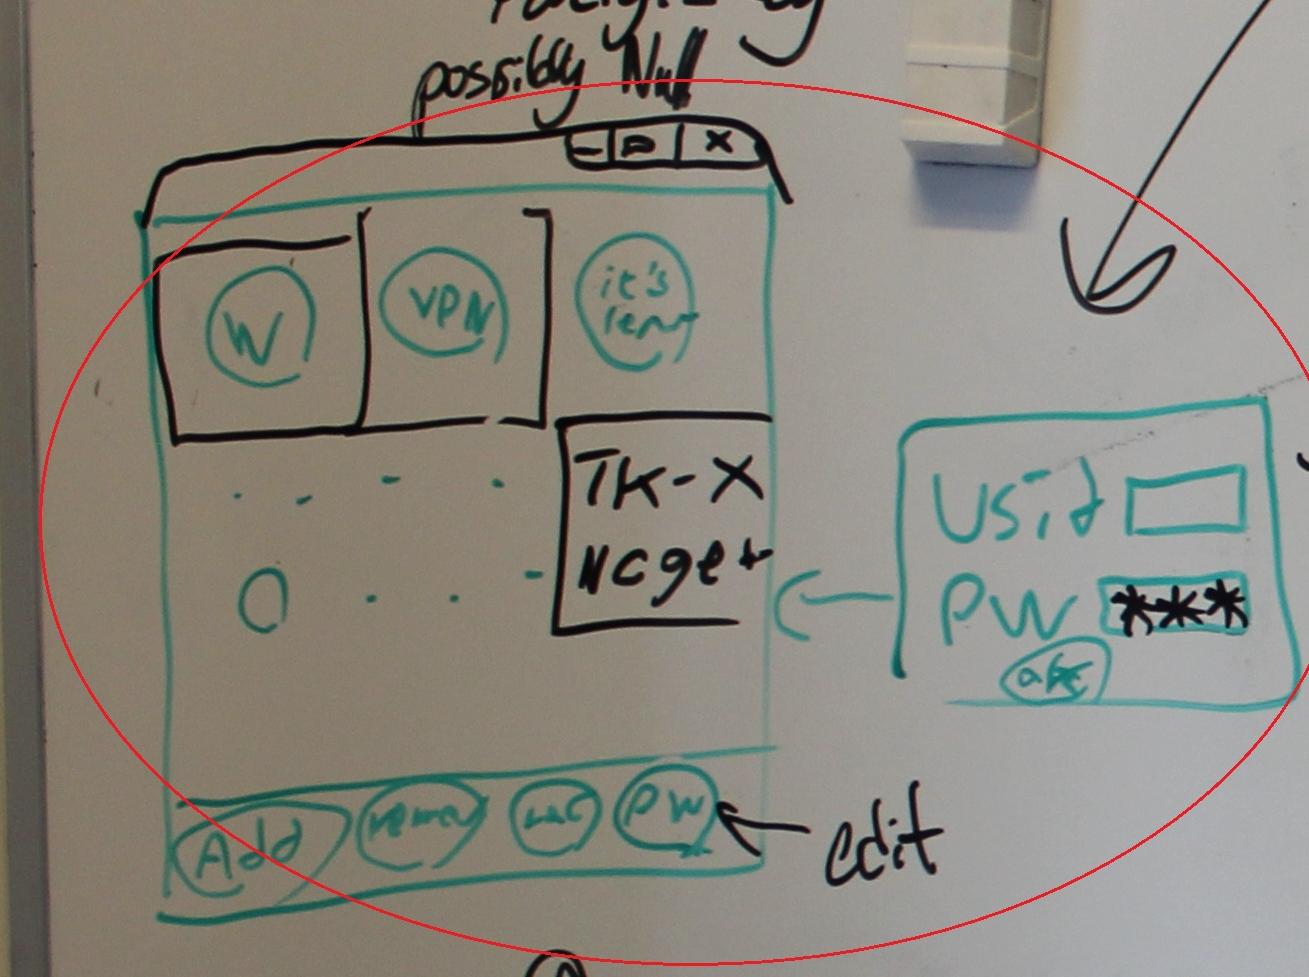
\includegraphics[height=150px]{Program-Design.png} 
\caption{Se appendix side \pageref{designbrain} for det fulde billede} 
\end{figure}

Dette har hjulpet os med hurtigt at kunne diskutere forskellige ideer og
koncepter, bl.a. hvordan brugergr�nse fladen skulle se ud, og for at skabe
overensstemmelse i gruppen med, hvordan designet skulle ende med at se ud. Da
vi s� havde besluttet os p� et design, i Low-Fidelity, kunne vi s� implementere
det i vores High-Fidelity, og derefter diskutere designet fuldkomment, og
eventuelt lave flere af disse iterationer, indtil vi f�lte, vi havde behov for
bruger input igen.

{\bf High-Fidelity prototyping}

% De var interaktive programmer, med faket funktionalitet
Efter vores andet interview med Martin og Martin (to l�rere p� Aarhus Tech),
      valgte vi at videreudvikle en High-Fidelity prototype baseret p� den kode
      vi havde fra Low-Fidelity prototypen. Idet vi vurderede, at en High-Fidelity
      prototype ville give os bedre feedback l�ngere ind i projektudviklingen,
      end flere Low-Fidelity prototyper. Dette gav mening for os, da vi nu havde
      f�et synspunkter fra forskellige brugere, og dette lod os lave et mere
      veldefineret design.

Den nye prototype kunne derefter indeholde de ting, der viste sig at v�re
n�dvendige. Som et specifikt eksempel, lagde vi m�rke til, at den ene l�rer
(under andet interview) per instinkt klikkede {Enter}, for at ville logge ind
efter at have skrevet sit brugernavn og password.  Da der ikke skete noget, gik
det lidt i st�.  P� denne m�de fandt vi tavs viden, som tillod en v�sentlig
forbedring i vores prototype, og kunne benyttes til at udvikle prototypen i den
retning, som brugerne benyttede den.

Vi fik desuden meget feedback, p� brugergr�nse fladen, som blev beskrevet som
'for teknisk', og med for meget (for brugeren) ligegyldig information, dette
f�rte os til at bede brugeren om at komme med deres vision for prototypens
brugergr�nse flade, hvilket vi s� kunne implementere til den anden prototype.

P� denne m�de, igennem en iterativ fremgangsm�de, lavede vi flere iterationer af
prototypen, som hver gang kom n�rmere brugerens �nsker og behov.

Vi har i alle de senere prototyper, lavet High-Fidelity, hvor mere og mere
funktionalitet er blevet tilf�jet, samtidig med at GUI'et er kommet t�ttere og
t�ttere p� det, brugeren �nskede.

{\bf Iterativt design}

% Er ogs� et krav i projekt beskrivelsen at prototype er udviklet over flere
% iterationer
Som n�vnt ovenfor, har vi arbejdet iterativt med brugeren, s�ledes at deres
feedback har direkte aff�dt �ndringer i vores High-Fidelity prototype, igennem
flere iterationer. Den iterative udvikling kan da ogs� ses i proces afsnittet.

Ud over vores direkte iterative design med brugerinddragelse har vi ogs�
skrevet koden vha. en iterativ arbejdsform.  Vi har lavet mange sm� iterationer,
        s�ledes at hver feature er blevet testet mange gange under selve
        udviklingen.

{\bf Contextual interview}

% Is this contextual interview?

Vores prim�re brugerkontakt har v�ret i gennem interviews, som vi har benyttet
til at diskutere problemstillinger, at afpr�ve prototyper, at f� feedback p� den
aktuelle prototype. 

Det har fungeret utroligt godt for os, at benytte kontekstuelle designs p� denne
m�de, idet vi har kunnet integrere brugeren, som en essentiel del af
udviklingsprocessen, og idet, at der har v�ret meget kort fra os, som udviklere,
    til brugeren, og dennes behov og holdninger.

Netop, at der har v�ret s� kort imellem os (s�vel fysisk, som logisk), har ogs�
gjort det muligt for os at interviewe brugeren igen, s� snart der var
sp�rgsm�l i udviklingen, som vi ikke selv havde mulighed for at vurdere, eller
afg�re.

Som supplement til dette har vi ogs� haft aktiv email korrespondance, n�r det
drejede sig om mindre beslutninger, eller opklarende sp�rgsm�l, hvor et
decideret interview ville have v�ret 'overkill'.

% Internt brugt i gruppen
{\bf User Experience Design}

Meget vigtigt for designet, er, at der skabes f�rre gener for brugere i forhold
til deres nuv�rende.  Derfor har vi under udviklingen lagt v�gt p�, at vores
l�sning laver s� f� irritationer hos brugeren som muligt, og derved skabe en
forbedret oplevelse i forhold til det eksisterende system.  Dette inkluderer
b�de de problemer, der uundg�eligt opst�r, n�r nye brugere skal l�re programmet
for f�rste gang, eller hvor meget der skal til for at bruge det, n�r det er sat op, og
hvor meget opm�rksomhed programmet kr�ver.

Vi har i processen valgt at designe efter, at brugeren skulle f�le instant
familiaritet med produktet, alts�, vi �nskede, at brugeren skulle f�le, at
produktet var lige til at g� til.

Vi har blandt andet opn�et dette ved at designe vores produkt, i stil med
hvordan andre programmer, som personalet allerede bruger, er designet.  Derudover
har vi valgt at s�tte stor fokus p� at anvende piktogrammer og ikoner, som
allerede har en fast betydning for brugeren, p� denne m�de beh�ver vi ikke
forklare brugeren noget eksplicit, da piktogrammet implicit forklarer det for
dem.

Et oplagt eksempel er tilstands-symbolet, der skifter fra et r�dt-kryds (ved
        fejl tilstand), til et orange/gult tandhjul (ved forbindelses- /
            arbejds- tilstand), og endelig til et gr�nt flueben (ved forbunden /
                oprettet tilstand).

Derudover har vi fokuseret p� at have rene og simple brugerflader, hvor kun
det allermest n�dvendige pr�senteres til brugeren, og hvor der ikke findes
uendeligt lange og komplicerede konfigurationsmenuer.

Endelig har vi fors�gt at f� vores prototyper til at 'passe' ind, i Windows
gr�nsefladen, og hvordan denne normalt fungerer, f.eks. kan programmet
minimeres til et Windows tray icon, s�ledes at det er gemt af vejen, og kun
komme frem, n�r der er behov for det, ligesom brugeren ville forvente det af
ethvert andet Windows service program.

{\bf Scenarie}

% Brugte scenarier da vi diskutterede design
Vi har i udviklingsprocessen brugt scenarie, b�de i form af use-cases, men ogs� i form af
stories, der fort�ller en mindre historie om den kontekst, hvor produktet bliver
brugt, og hvordan det bliver brugt.

Vi har derudover internt arbejdet med abstrakte konceptuelle scenarier, som
overordnet set beskriver brugs-situationen, og brugs-m�nstre for vores produkt.

{\bf Use Case}

% Use case er en beskrivelse af en interaktion i mellem en Actor (bruger) og
% systemet.
Vi har i vores udviklingsproces haft fokus p� use-cases, s�ledes at vi for
enhver feature i systemet altid har haft en id� om, hvordan den specifikke
feature ville komme i brug, og hvem, der ville bruge den. 

Dette har hjulpet til at sikre, at alle programmets features og funktioner
faktisk har en aktuel brugssituation tilknyttet, og dermed er relevant for det
endelige produkt.

Og p� samme m�de har det ladet os eliminere de dele af user-interfacet, som har
vist sig at v�re ubrugelige, idet, der ikke har v�ret nogle use-case tilknyttet,
     og da det ikke har v�ret muligt, at komme p� et use-case.

Det oplagte eksempel fra vores udvikling proces er 'Opdater' knappen, som
brugeren aldrig vil have en grund til at klikke p�, og derfor b�r fjernes fra
produktet, i den n�ste iteration (den som ville komme efter rapportens
        aflevering). - Eftersom knappen hermed ikke har nogen duelig
specifikation


Vi sendte emails ud til flere skoler for at pr�ve at starte et samarbejde.
Lars Lisberg, IT-teamleder ved Aarhus Tech, skrev tilbage, at de var
interesserede i et samarbejde.  De havde et �nske om udvikling af et s�kaldt
single-sign-on system, s�ledes at de mange services som ansatte benytter, kan
logge p� en gang, centralt, s� der herefter er adgang til alle services.  Vi
aftalte herefter et interview med Lars for at arrangere termerne, hvorp�
projektet vil fungere, og hvilke krav de stiller for en eventuel l�sning.
For at afd�kke disse sp�rgsm�l forberedte vi et interview, som kan ses i
appendixet side \pageref{interview1}

%med Lars Lisberg, IT-teamleder ved Aarhus Tech.

Vi valgte at optage dette interview p� film, for at kunne bruge det til

eventuelle senere afleveringer, og for at kunne behandle svarene senere.
Vi startede interviewet med at lave en observation af, hvordan den aktuelle
arbejdsgang fungerer, for at f� en generel ide om omfanget af problemet,
herefter udf�rte vi vores interview, for at f� besvaret vores sp�rgsm�l.
Vi kom frem til, at den prim�re m�lgruppe for systemet er de ansatte p� Aarhus
Tech, og i mindre grad eleverne, og vi har derfor i f�rste omgang besluttet prim�rt at designe efter
medarbejdernes behov.
Baseret p� dette f�rste interview, og de informationer vi fik, begyndte vi at designe
en Low-Fidelity prototype, som havde til form�l at formidle vores umiddelbare forslag til en l�sning.

\begin{figure}[ht]
\centering
    \begin{subfigure}[b]{0.35\textwidth}
    \centering
   	\includegraphics{1.Prototype/Login_Vindue}
    \caption{Login vindue}
    \label{s�renslortebillede2}
    \end{subfigure}
    \begin{subfigure}[b]{0.6\textwidth}
    \centering
   	\includegraphics[height=200px]{1.Prototype/Status_Vindue}
    \caption{Status Vindue}
    \label{s�renslortebillede3}
    \end{subfigure}
    \caption{}
    \label{s�renslortebilleder}
\end{figure}

Som det ses p� \autoref{s�renslortebilleder}, var f�rste prototype meget skrabet.
Den bestod af et Login vindue(som ses p� \autoref{s�renslortebillede2})
hvor brugeren skulle indtaste brugernavn og adgangskode for derefter at blive sent videre.
Herefter ville brugeren se et vindue(\autoref{s�renslortebillede3})
der indeholdte en liste over de forskellige services og information om hvorvidt denne service havde forbindelse eller ej.


For at f� bekr�ftet Lars Lisbergs teori om at de mange logins skaber
irritationer og problemer hos medarbejderne, kontaktede vi Aarhus Tech igen og
bad om at f� et interview.  Denne gang med to l�rere.  Under interviewet ville
vi ogs� gerne se hvordan en l�rer benytter det nuv�rende system, og pr�senterede
dem for den vores f�rste prototype.  Her sigtede vi efter at f� feedback, der
kunne hj�lpe til med at forbedre designet.\\


%{\bf Interview 2, 23/04} med Martin og Martin, to l�rer ved Aarhus Tech.
Efter interviewet lavede vi i gruppen en opsamling, hvor vi skrev ned, hvordan de
sp�rgsm�l, som vi havde forberedt, var blevet besvaret.  Her fik vi bekr�ftet af
de to l�rere, at de mange forskellige logins er et egentligt problem.

I det feedback vi fik, var der et generelt �nskede om en p�nere og
mere brugervenlig brugergr�nseflade.
Desuden �nskede de, at systemet kunne blive mere brugerstyret, s�ledes at brugerne selv kunne tilpasse, hvilke
servies der var aktuelle for dem, samt at konfigurere disse med deres personlige brugernavn og password, uden at IT afdelingen skulle indblandes.
Vi kunne alts� konkludere, at vores brugergr�nseflade skulle redesignes, og vores model af, hvilken rolle brugeren spiller ifht. administratoren, ogs� skulle
revurderes.
Med hensyn til brugergr�nsefladen havde vi af den ene af l�rerne f�et et
specifikt forslag til designet, hvor hver service skulle repr�seneres ved et
logo med et lille pictogram, som skulle vise servicen�s tilstand. 
Vi diskuterede i gruppen, hvordan vi skulle redesigne brugergr�nsefladen.
Vi brainstormede ved at tegne udkast til et design p� en tavle.

\autoref{figsdesign} der viser vores to prim�re ideer.


\begin{figure}[ht]
\centering
    \begin{subfigure}[b]{0.45\textwidth}
    \centering
   	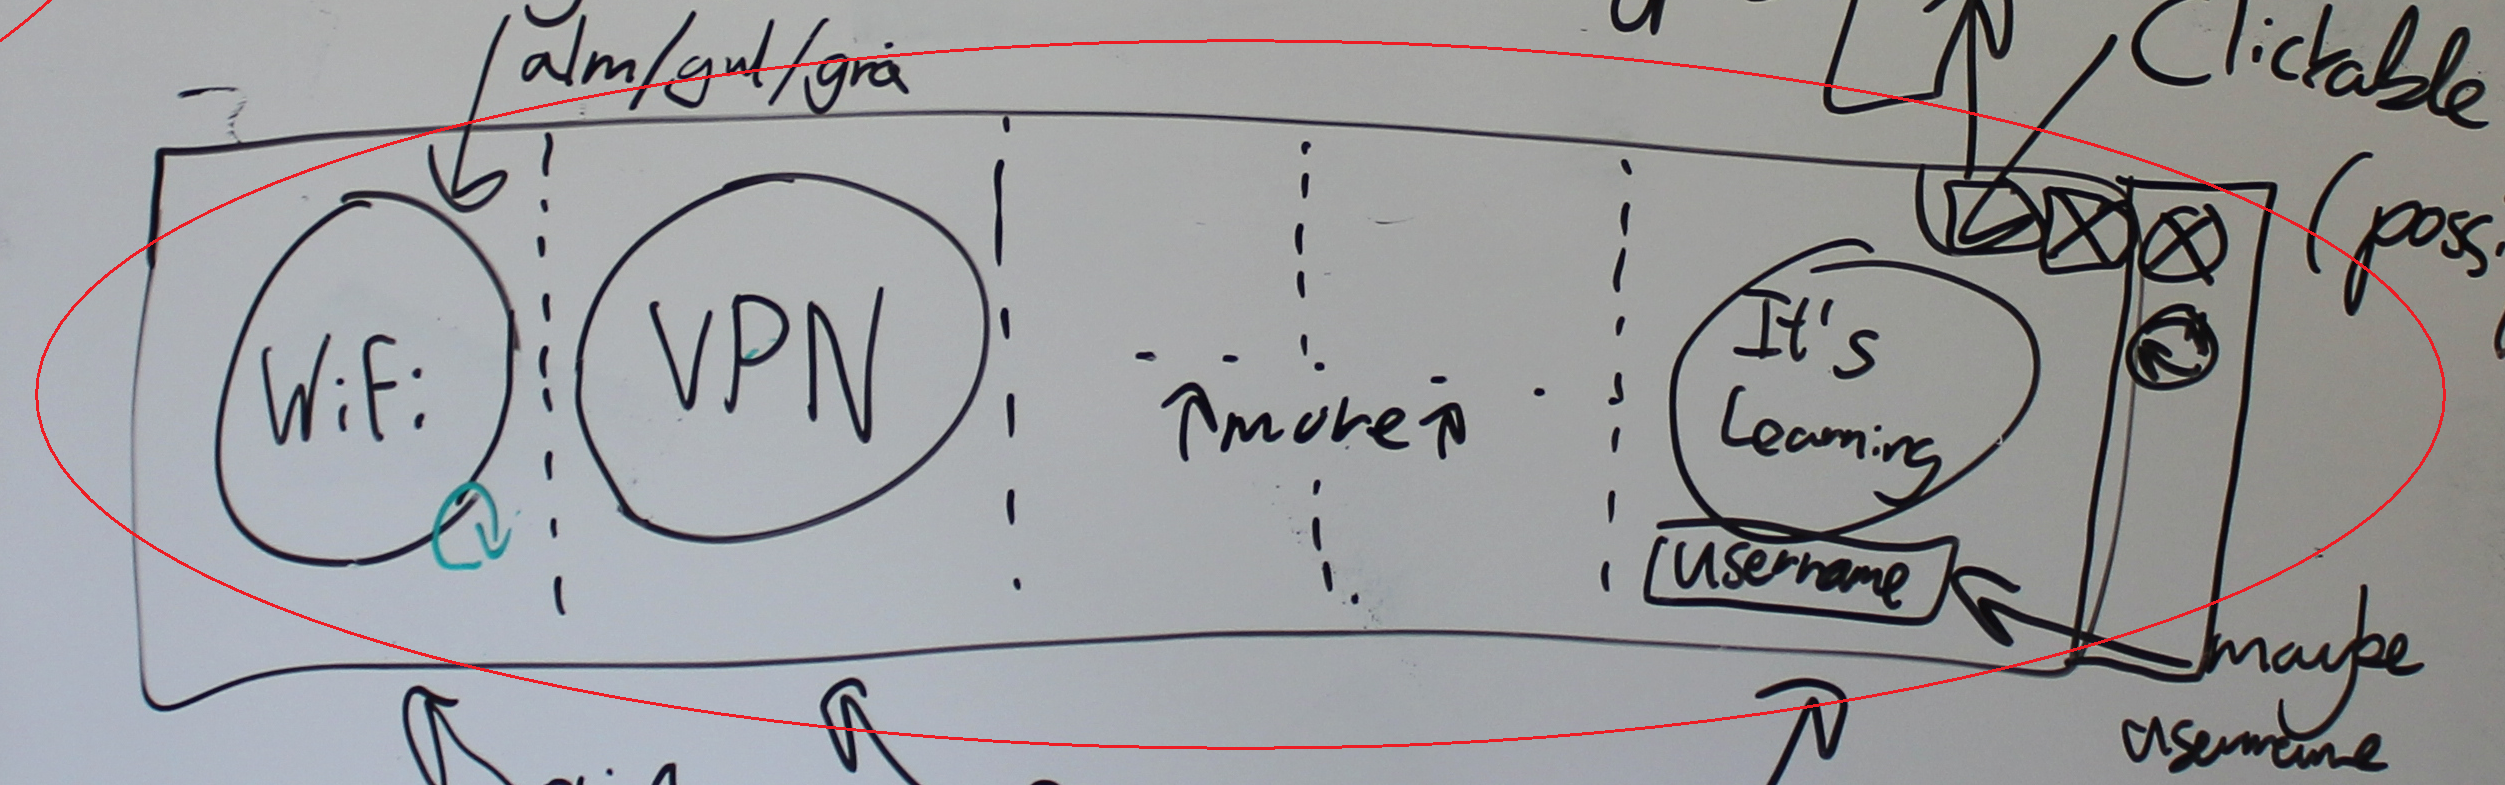
\includegraphics[width=\textwidth]{Web-Design}
    \caption{web design}
    \label{figsdesign1}
    \end{subfigure}
    \begin{subfigure}[b]{0.45\textwidth}
    \centering
   	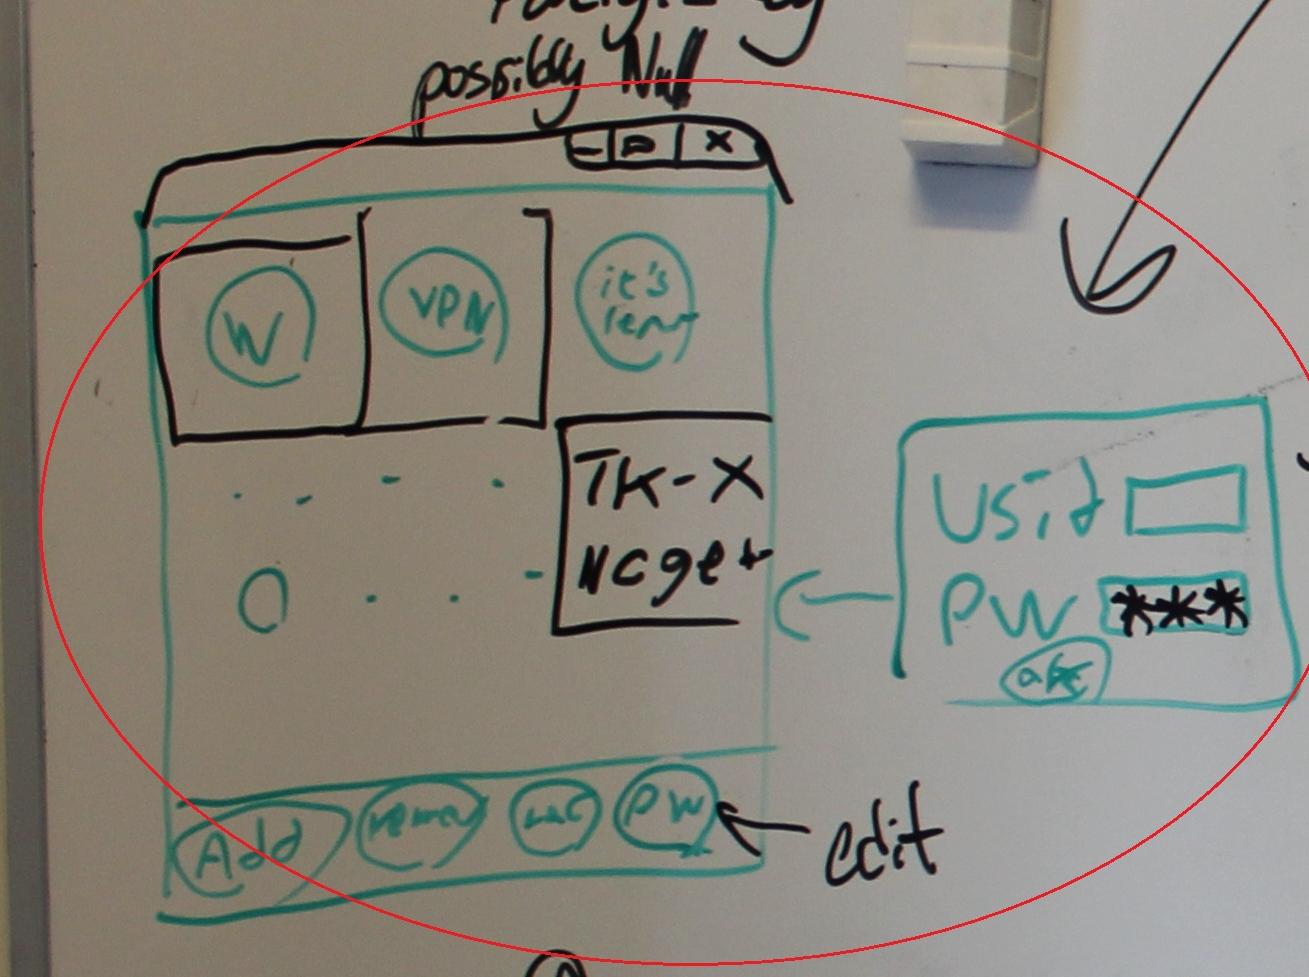
\includegraphics[width=\textwidth]{Program-Design}
    \caption{program design}
    \label{figsdesign2}
    \end{subfigure}
    \caption{Se appendix side \pageref{designbrain} for fulde billede}
    \label{figsdesign}
\end{figure}

Som det ses p� \autoref{figsdesign1}
bestod en af vores ideer af en horisontal menubar, hvor ikonerne for de forskellige services var linet op efter hinanden.
I dette design ville hvert ikon have et pictogram nede i h�jre hj�rne, der angav dennes status.
Dette design forkastede vi dog, da det mere mindede om et design til en web applikation, og vi t�nkte, at dette muligvis ville forvirre brugerne. 
Ydermere havde vi problemer med at placere funktionsknapperne i programvinduet.
I stedet gik vi, som det ses i \autoref{figsdesign2}
over til et mere klassisk look.
Dette design best�r af et tiln�rmelsesvis kvadratisk programvindue, hvori ikonerne for de forskellige services er linet op i en matrix.
I bunden af vinduet finder man funktionsknapperne.
Da dette var et mere traditionelt look, og ville komme til at ligne programmer, som brugerne havde brugt f�r, ville det intuitivt set v�re nemmere for brugerne at finde rundt i.
Vi tog dette grunddesign og arbejde videre med det.

\begin{figure}[ht]
\centering
   	\includegraphics[height= 150px]{IMG_3176}
    \caption{}
    \label{s�renslortebillede1}
\end{figure}

Som det kan ses p� \autoref{s�renslortebillede1}, tegnede vi en meget basic sekvensmodel, 
der viser, hvordan en bruger logger ind for derefter at komme til et statusvindue med ikoner for de forskellige services, og funktionsknapper i bunden.
Login vinduet valgte vi at beholde fra den f�rste prototype, da den p� en overskuelig m�de klarede login processen.
Funktionsknapperne i statusvinduet bestod af en add-knap, der tilf�jer services til statusvinduet.
remove-knappen fjerner services fra statusvinduet.
Ydermere er der en re-connect-knap, en password-knap, der ville s�tte password og brugernavn for en service, en refresh-knap der opdaterer status for de individuelle services og en logout-knap.
Ved at trykke p� logout knappen, vil brugeren blive sendt tilbage til Login vinduet.

Dette design blev grundlaget for vores redesign af GUI'en 


Herefter diskuterede vi administratorens rolle, ifht. brugeren, og hvordan vi
kunne f� gjort det muligt, at brugeren er den eneste, der arbejder med sit eget
brugernavn og kodeord.  Vi endte med at lave en tydelig deling af ansvaret,
           s�ledes at ops�tning af generelle parametre for services, samt hvilke
           services en given bruger kan tilg�, klares af administratoren.
           Ops�tning af brugernavn og kodeord, samt hvilke services der skal
           vises for brugeren, klares af brugeren selv.  For at f� uddannet
           brugeren i netop dette, ville den ene af l�rerne Martin, der ogs� er
           teknisk ansvarlig, kunne holde et info-m�de, samt eventuelt skrive en
           mindre tutorial.

\begin{figure}[ht]
    \centering
   	\includegraphics[height=200px]{2.Prototype/Status_Vindue}
    \caption{Status Vindue}
    \label{s�renslortebillede4}
\end{figure}

Da vi havde besluttet designet, gik vi i gang med revidering af prototypen, der
skulle inkludere vores 'status vindue', der ses p� \autoref{s�renslortebillede4}, som l�rerne havde efterspurgt, desuden
besluttede vi, at vi nu �nskede at integrere en del funktionalitet i denne
prototype. Dermed gik vi fra en Low-Fidelity prototype og til at udvikle en
high-fidelity prototype.  Dette gjorde vi, da vi vurderede, at s�dan en
prototype ville kunne give os bedre feedback, p� lang sigt. Som vi gjorde
i den f�rste prototype, har vi til at realisere vores design, besluttet os for
at benytte 'Java swing' til at skrive GUI.  For ops�tning og administration har
vi valgt at bruge en MySQL server, da Lars Lisberg informerede os om, at det var
en teknologi, som de allerede havde til r�dighed.

Vi besluttede, at funktionaliteten, mht. at oprette forbindelse til Wi-Fi, og
VPN, nemmest implementeres ved at benytte Windows programmerne til dette, og vi
har derfor skrevet kode, der kalder disse programmer.  Dette betyder, at
l�sningen kun fungerer p� Windows. At systemet til at starte med kun vil fungere
p� Windows er udm�rket, da medarbejderne af Aarhus Tech f�r udleveret
arbejdscomputere, der alle k�rer Windows.  Enkelte medarbejdere benytter egne
computere, og disse k�rer styresystemer efter brugerens �nsker.  Set i lyset af
den tidsramme vi arbejder indenfor, blev vi med Lars enige om, at vi i f�rste
omgang skulle fokusere p� Windows.

For at muligg�re, at man kan tilg� HTML services, som fx de mange cloud services
medarbejderne benytter, har vi implementeret en l�sning i Java vha. 'apache
httpclient' biblioteket\footnote{\citep[]{httpclient}}. Denne kan logge ind,
og vi har dermed kun udfordringen med at f� overf�rt cookien fra dette login
til brugerens browser. For at klare denne opgave har vi diskuteret flere
mulige l�sninger;
\begin{itemize}
\item Automatiseret browser-import af cookies
\item HTTPS Session Hijacking
\item HTTPS Proxy (der laver requests p� brugerens vegne).
\end{itemize}
Hver af disse har deres fordele og ulemper, som vi har diskuteret.  Vi valgte at
benytte os af HTTPS Proxy'en, som, omend den har en del problemer, syntes at
kunne l�se vores problemstilling.  Desuden vil l�sningen med en proxy-server
v�re browser uafh�ngig, idet den vil svare brugerens browser, som enhver anden
webserver ville g�re det.  Kun ops�tningen vil v�re browser specifik, men da den
prim�re browser for de ansatte, er internet explorer, er dette et mindre
problem. 

Vi begyndte herefter at forberede et interview af Lars, for at finde svar p� nogle
nogle af de tekniske sp�rgsm�l, der var kommet op i udviklingen af vores
reviderede prototype, eksempelvis; Om �bne licenser ville v�re et problem,
           information om det netv�rk, der i fremtiden skal udskifte VPN
           systemet, samt til hvordan systemet skal administreres. Derudover
           var vi n�dt til at f� afklaret hele sikkerhedsproblemet omkring
           systemet; hvem vi kan forvente at kunne stole p�, hvor stor sikkerhed
           der er n�dvendig, hvor ofte dom�ne kodeordet skiftes, osv.
%{\bf Interview 3, 07/05} med Lars Lisberg, IT-teamleder ved Aarhus Tech.

Under dette, tredje interview, blev det klart for os, at vores system, som
�nsket af l�rerne, ville kunne integreres med det eksisterende Active Directory
system, s�ledes at single-sign-on systemet, automatisk starter op, og kommer til
den aktive tilstand, som en del af Windows login proces.  P� denne m�de ville
brugeren kun skulle logge ind p� sin Windows bruger og ikke som tidligere
tilt�nkt, logge p� maskinen, og herefter p� logge p� single-sign-on systemet.
Det automatiske login vil desuden v�re sikkert, da Active Directory m� antages
at v�re sikkert.  Vi er endvidere blevet opm�rksom p�, at ops�tning af proxy,
   certifikater og lignende ikke vil v�re noget problem, da dette kan rulles ud
   vha. Active Directory, og da eventuelle problemer vil v�re rimeligt low-tech,
   som den IT ansvarlige og l�rerne imellem nemt skulle kunne l�se.  Under
   interviewet fandt vi derudover ud af, at vi som udgangspunkt kan stole p� IT
   afdelingen, men at vi dog skal s�rge for, at kodeord i databasen ikke kan
   l�ses i plain-tekst.  Mht. administration, syntes Lars godt om fordelingen
   imellem brugerens og IT afdelingens ansvarsomr�der, idet IT afdelingen p�
   denne m�de slipper for at skulle indf�re brugernes personlige brugernavn og
   kodeord. Mht. IT administrationssiden af administrationen, ville de gerne have
   simple SQL scripts, som de kunne k�re fra deres Active Directory triggers.
   Vi blev dog sammen med Lars enige om, at vi, mens kurset k�rte, prim�rt skulle
   fokusere p� brugerdelen af systemet, og at vi kunne arbejde videre med
   administrationsdelen i et eventuelt videre forl�b efter kurset var afsluttet
   Mht. licens udtrykte Lars intet problem med brugen af open-source licenser,
   tv�rtimod mente han, at det ville g�re det nemmere for dem at kunne
   udlicitere vedligeholdelse af systemet.
%% MARKER Onsdag d. 08/05:�

Efter interviewet med Lars har vi kigget n�rmere p�, hvordan et proxy
autokonfigurationsscript ser ud, og vi har udviklet et s�dan, der blot kan
loades ind i brugernes browser, hvorefter proxy'en automatisk vil blive
konfigureret.  Disse scripts er standardiserede, og vil derfor virkee p� alle
browserne.  N�r det kommer til ops�tning af certifikater, har vi eksporteret et
certifikat, som kan installeres ved et simpelt dobbelt klik, og en tur igennem
en import wizard.  Dette vil fungere for Internet Explorer, men metoden med at
loade certifikater er browserspecifik, og man er derfor n�dt til manuelt at loade
certifikatet, hvis man �nsker at benytte en anden browser.  I arbejdet med
prototypen har vi fortsat implementeringen af vores GUI.  Vi har bl.a. f�et
opbygget funktionalitet bag de forskellige knapper, s�ledes at knapperne �bner
de forventede vinduer, eller de kalder de forventede funktioner.

Mht. at implementere vores http services, har vi kigget p� forskellige proxy
l�sninger;
\begin{itemize}
\item The Grinder
\item Burp Proxy
\item Charles Proxy
\item mitmproxy
\item mitmproxy (Java projektet)
\item honeyproxy
\item tlsproxy
\end{itemize}

Hver af disse proxy'er har vi vurderet, og vi stod med et valg mellem 
to mulige l�sninger.  Enten skulle vi benytte en central UNIX server, som skulle
klare alle proxy forbindelser, denne ville s� k�re 'mitmproxy'.  Ellers skulle
vi benytte Tlsproxy, og l�re go og samtidig tilf�je to programmeringssprog til
projektet.  Vi var dog s� heldige, i sidste �jeblik, at falde over et andet
alternativ, i form af 'exproxy, der er et Java program bibliotek, der kunne l�se
opgaven\footnote{\citep[]{exproxy}}. Ved skriftlig henvendelse til udvikleren af
exproxy, er det lykkedes at f� udleveret source-koden, under apache open-source licensen,
s�ledes at denne kan modificeres og tilpasses, hvis prototypen kr�ver dette.  I
implementeringen af exproxy, i resten af projektet, har vi valgt at redesigne,
hvordan proxy serveren skal fungere.  Oprindeligt var det tilt�nkt, at vi ville
lave en http request p� brugerens vegne, og herefter returnere svaret herfra,
     til brugeren.  Med det valgte program bibliotek har det vist sig, at det
     simpelthen er muligt, blot at �ndre p� den http request, som brugeren
     sender, s�ledes at denne bliver lavet om til en login request.

%Vi har desuden brugt en del tid, p� at rydde op i koden, for forbedre den
%eksisterende kode, f.eks. havde vi i den anden prototype, valgt, at benytte et
%'JTable' i koden til at vise services i status vinduet, men da dette ikke var
%beregnet til at blive brugt p� denne m�de besluttede vi at erstatte det med en
%'JList', som bedre passede p� den funktion vi �nskede at udf�re. F.eks.
%tilpasses denne 'JList' st�rrelsen automatisk efter programmet vindue, imens
%programmet k�re, s�ledes at status vinduet kan resizes uden problemer.

%Vi kunne ved �ndringen fra 'JTable', til 'JList' desuden fjerne n�sten 100
%linjer kode, s�ledes at koden blev mere vedligeholdig for fremtiden.

%Det er vigtigt, at bem�rker, at dette udelukkende var en refaktorering, s�ledes
%at brugen faktisk ikke opdagede �ndringen, idet brugergr�nsefladen var n�sten
%fuldkommen ens.

Vi valgte at redesigne hele systemet til at benytte et centralt 'Event system',
   frem for at alle klasser direkte kontaktede dem, der skulle udf�re en given
   opgave. P� denne m�de kunne vi decouple de forskellige klasser, (f�rre
           referencer de forskellige klasser imellem), hvilket har resulteret i
   en langt mere fleksibel og dynamisk kodebase, hvor alle klasser blot fort�ller,
   hvilke events, der er aktuelle for dem, og s� reagerer, n�r de modtager disse
   events. De klasser, der �nsker at fort�lle, at noget er sket, simpelthen blot
   laver en event, til at fort�lle dette, til dem (omend nogle), der er
   interesserede.

Dette eventsystem gjorde os endvidere i stand til, at udvikle de forskellige
dele af prototypen i parallel, og s�gar undlade specifikke dele af prototypen,
     uden nogen problemer. Eksempelvis, kom SQL updater systemet f�rst efter
     tredje og sidste fremviste prototype.

%Desuden frigjorde eventsystemet fra at skulle redigere i de gamle filer, om og
%om igen, n�r noget skulle tilf�jes, f.eks. koden til at h�ndtere hvad der sker,
    %n�r en knap trykkes. - Dette hjalp os med at undg� at introducere bugs i
    %det fungerende kode.

Vi har herefter arrangerede vi vores fjerde interview, for at kunne fremvise
vores 'endelige' funktionelle prototype, som nu var blevet f�rdig, vores �nske
var, at fremvise prototypen og dens funktionalitet for brugere.

Vi �nskede desuden at danne os et endeligt indtryk af, om prototypen var klar til
distribution, eller om prototypen burde revideres yderligere.

%{\bf Interview 4, 24/05} med Martin, Martin og Karin, to l�rer og en
%uddannelses leder ved Aarhus Tech.

Interviewet gav hovedsageligt positivt feedback, men der kom ogs� noget
konstruktiv kritisk.  Blandt andet blev det klart, at Opdater knappen er
forvirrende for nogle brugere.  Brugerne kunne ikke forklare os, hvad knappen
gjorde, og vi havde faktisk ogs� problemer med at forklare det.  Der var ogs� et
�nske om at adskille system services (Wi-Fi, VPN, osv.) fra de andre services.
Yderligere kom der et forslag om at tilf�je muligheden for, at brugere kunne
oprette ikoner p� skrivebordet for hver af de services, der er logget p� gennem
single-sign-on systemet.

Da kurset nu er ved at v�re f�rdigt, har vi endnu ikke evalueret eller implementeret de ovenst�ende forslag til forbedringer.
Derudover er der en r�kke andre ting, der ogs� stadig mangler at blive implementeret, inden vi vil have et f�rdigt produkt.
Disse punkter kan ses i backloggen som findes i appendixet side \pageref{backlog}.


\newpage
\section{Brugersamarbejde}
Da vi startede projektet, havde vi kun en email fra Lars Lisberg at g� efter, 
vi vidste meget lidt om hvilke forventninger de fremtidige brugere ville have, og inten om deres eksisterende system.
Til det f�rste interview var det derfor meget vanskeligt at komme med dybteg�ende sp�rgsm�l, 
vi bestemte os for at kontekstuelt interview, hvor vi bedte Lars Lisberg om at vise deres eksisterende login system, og pr�ve at vise hvordan det er problematisk.
For at forberede os selv til at uddybe interviewet, var vi n�d til at g�tte p� hvordan deres system virker, 
fra tidligere erfaring, s� vi have noget at lave vores sp�rgsm�l fra.
Ud fra dette ville vi pr�ve at finde de centralle tekniske krav, dvs. den funktionalitet som er n�dvendig uanset brungergr�nseflade,
og de resurser der er tilg�ngelige fra Aarhus Tech, vi havde f.eks. en ide om at en SQL server kunne blive n�dvendig.
Fordi vi manglede s� meget information, besluttede vi at vente med at udvikle nogen form for prototype indtil efter det f�rste interview.

Det f�rste interview gav en masse brugbar information, vi fik ogs� svaret p� nogle af de sp�rgsm�l vi havde forberedt, selvom mange af dem var meget vage. 
Desv�rre var nogle af de sp�rgsm�l ikke s� relevante, efter at have set deres eksisterende system.
Vi havde ikke forventet at systemet kun skulle bruges af ansatte, vores forestilling var at det skulle bruges af alle med internet adgang ved Aarhus tech.

Fordi vi nu havde nok information til at lave en low-fidelity prototype, begyndte vi at skifte fokus til at lave prototyper, i stedet for kontekstuelle interviews.
I det andet interview brugte vi dog ogs� kontekstuelle interview igen, hvor vi fik Martin og Martin til at vise deres normalle login process frem.
Ideen her var at vi derved kunne bekr�fte det Lars Lisberg havde sagt, og f� et andet synspunkt i, hvor slemt et problem det egentligt er, som vi arbejder med.

Den ene l�rerer sagde at han skulle logge ind 25 gange om dagen, og han ofte skulle logge ind igen hvis han bev�ger sig fra et lokale til et andet. 
Det var mere end vi havde forestillet os, og fik os til at udvide Simple-SignOn til ogs� at logge ind i WiFi og VPN netv�rk automatisk.
Vi blev ogs� overrasket, da han, efter at have skrevet brugernavn og password ind i Simple-SignOn, pr�ve at logge ind ved at trykke Enter, 
det er noget vi ogs� g�r ofte, men helt havde overset i vores design indtil vi s� det.
Det feedback vi fik, gjorde ogs� en stor forskel i det grundl�ggende design, de to l�rere sagde at de gerne ville have mere kontrol over det, 
hvilket �ndrede meget p� hvordan senere prototyper kom til at se ud.

Det ekstra brugerinput til designet af Simple-SignOn har klart resulteret i et bedre design, 
vi havde ikke forudset at brugere gerne ville styre hvilke services de bruger, hvis ikke det var blevet sagt til et interview.

%TODO: hvordan 
Efter det andet interview, lavede vi ikke l�ngere observationer af det eksisterende login system, i stedet var fokus nu p� prototyping.
Vi mente at vi havde f�et nok bruger feedback til at lave en mere konkret prototype, 
og vi gik derfor fra low fidelity prototype tests til high fidelity.

Fra det andet interview, sagde den ene l�rer at de er ved at udskifte deres VPN system med et seperat WiFi netv�rk, 
det havde vi ikke h�rt noget om fra Lars Lisberg, og det lavede en del forvirring.
Da Simple-SignOn kr�ver administration, talte vi i gruppen om hvordan dette skulle g�res.
Fordi vi ikke havde noget grundlag for at beslutte hvor kompleks s�dan en l�sning kunne v�re,
%TODO: reference til andet sted i rapporten om sikkerheden, brug evt. \pageref
og desuden pga. sikkerheds beslutninger og andet, 
f�lte vi det n�dvendigt at lave endnu et interview med Lars Lisberg, med fokus p� disse punkter.
Vi havde ogs� en ny prototype klar p� tidspunktet, og besluttede os for at vise den frem, 
vi valgte at vise den f�rste prototype og derefter den anden, fokus var dog statig p� det administrative og tekniske.

Til det administrative havde vi i gruppen, talt mest om de to 'ekstremer', en GUI som klarer det eller manuelle SQL queries. 
Under interviewet kom vi frem til at det burde g�res via scripts, som er lidt i mellem de to ekstremer.
Med hensyn til prototyping under det trejde interview, s� fik vi kun meget lidt ud af det. Da vi viste den f�rste prototype frem, 
s� Lars Lisberg skuffet ud, som om han var overrasket over hvor lidt vi havde n�et. 
Fremvisning af den f�rste prototype gav meget lidt brugbart feedback, det f�ltes som en d�rlig ide, set i bakspejlet efter interviewet.
Det blev reddet, da vi derefter viste den anden prototype frem, s� han mere afslappet ud, feedback var derefter positivt, 
og han n�vnte at teksten i programmet m�ske burde v�re p� dansk, i stedet for engelsk, som vi er vandt til at skrive n�r vi laver programmer.

Hvis ikke vi havde f�et dette feedback, havde vi nok lavet et GUI til administration, 
og brugergr�nsefladen i Simple-SignOn var nok forblevet p� engelsk.



\newpage
\section{Scenarier af prototype}
% TODO: Beskriv via scenarie hvordan VORES prototype kommer til at blive brugt.
% Dette skal bruges til reflektion, og skal vise evt. fejl/mangler med den prototype vi afleverer.

F�rste senarie er en historie der omhandler en l�rer p� Aarhus Tech ved navn Martin, og hvordan han benytter den prim�re id� og funktionalitet ved Simple-SignOn. 
Meningen med dette senarie er kort at demonstrere de prim�re funktioner og problematikker, som systemet er t�nkt at skulle l�se.


Andet senarie omhandler en medarbejder p� Aarhus Tech ved navn Gitte, og hvordan hun, f�rste gang hun benytter programmet kommer igennem mange af funktionaliteterne. 
Dette senarie har til form�l at demonstrere den f�rste brug af programmet og hvordan det s�ttes op til brug.\\
Gennem denne demonstration, vil man f� et genneml�b af funktionerne i programmet, og man vil f� en id� om vores overvejelser omkring hvilke funktionaliteter Simple-SignOn skulle have.

\leavevmode \linebreak
{\Large Senarie 1:}
Martin(en l�rer p� Aarhus Tech) m�der om morgenen p� Aarhus Tech.\\
Da Martin i sidste uge var p� kursus i Kolding, skal han benytte Travel-X til at rapportere rejseomkostningerne forbundet med kurset. 
Travel-X ligger dog ikke direkte p� Martins arbejdscomputer, men i clouden.
Dette havde betydet, at Martin f�r i tiden f�rst skulle logge p� et tr�dl�st netv�rk, derefter logge p� VPN for til sidst at indtaste/huske sit brugernavn og kodeord til Travel-X. 
Alle disse indtastninger slipper Martin dog heldigvis for idag.
Da Martin benytter programmet Simple-SignOn som ligger lokalt p� hans computer, skal han blot �bne programmet, og �n gang indtaste sit brugernavn og adgangskode. 
Herefter kan han straks �bne Travel-X via et link i programmet og rapportere sine rejseomkostninger.\\ 


Da Martin ogs� st�r for at l�gge skema for de studerende, begynder Simple-SignOn for alvor at spare ham tid. 
I mods�tning til i gamle dage, hvor han nu skulle p� nettet for at tilg� Elevplan og her igen indtaste (forskellige fra de andre)brugernavn og adgangskode, kan han nu, da han er logget p� Simple-SignOn, blot trykke p� linket der repr�senterer Elevplan, og straks er han inde p� Elevplan, logget ind og klar til at arbejde.
Martin skal nu hen og undervise en klasse.
Inden han g�r, skal Martin huske at logge af de forskellige services, da der kan forekomme informationer som ikke skal v�re tilg�ngelige for eleverne.
Martin gl�dede sig endnu engang over Simple-SignOn, idet han nu blot beh�vede at trykke p� log ud knappen i programmet for at logge af alle services. 


\leavevmode \linebreak

Andet senarie omhandler en medarbejder p� Aarhus Tech ved navn Gitte, og hvordan hun, f�rste gang hun benytter programmet kommer igennem mange af funktionaliteterne. 
Dette senarie har til form�l at demonstrere den f�rste brug af programmet og hvordan det s�ttes op til brug.\\
Gennem denne demonstration, vil man f� et genneml�b af funktionerne i programmet, og man vil f� en id� om vores overvejelser omkring hvilke funktionaliteter Simple-SignOn skulle have.

\leavevmode \linebreak
{\Large Senarie 2:}
Gitte og hendes kollegaer havde lige v�ret til et informationsm�de, hvor de var blevet gjort opm�rksomme p� og havde f�et installeret et nyt program ved navn Simple-SingOn. \\
Skolens IT-vejleder Martin Hejgaard havde forklaret dem, at dette program havde til form�l at lette deres daglige arbejde. 
Dette ville programmet g�re ved at muligg�re, at brugeren kun skulle logge ind �n gang i forbindelse med at starte programmet, for derefter at have fuld adgang til alle de services som han/hun skulle bruge i l�bet af dagen. \\
Martin havde hjulpet dem med at installeret et certifikat i Internet Explorer og sat browseren til at benytte en bestemt proxy.\\
Nu sad Gitte p� l�rev�relset og skulle til at benytte programmet for f�rste gang.
Hun klikkede p� programmets ikon p� skrivebordet, og frem kom et lille vindue der bad hende om at angive brugernavn og adgangskode.
Dette gjorde Gitte, og hun havde ikke noget problem med at huske hverken brugernavnet eller adgangskoden, idet Martin havde fortalt dem, at disse var de samme som n�r de skulle logge ind p� Active Directory.\\


Efter at have skrevet sit brugernavn og adgangskode trykkede Gitte p� knappen i bunden af sk�rmen ved navn 'Forbind'.
Det lille login vindue lukkede ned, og i stedet �bnede et nyt lidt st�rre vindue.
Dette vindue havde tre ikoner i et statusvindue. Disse ikoner repr�senterede WiFi, DNS og VPN.
Hvert af disse ikoner havde et lille pictogram nede i deres h�jre hj�rne der tilkendegav hvor i forbindelsesprocessen de befandt sig.
F�rst fik de hvert et orange tandhjul, dette blev dog relativt hurtigt skiftet ud med et gr�nt flueben der tilkendegav, at der nu succesfuldt var oprettet forbindelse.\\


Da dette var f�rste gang Gitte havde �bnet programmet, indeholdte statusvinduet dog ikke ikoner, for nogle af de services hun gerne ville tilg�, men blot de tre tidligere n�vnte.
Dette g�ttede Gitte p�, at hun kunne �ndre p� ved at klikke p� knappen i bunden af vinduet ved navn 'Tilf�j'.
Ganske rigtigt, frem kom et nyt vindue der indeholdte en liste over alle de services der var tilg�ngelige for hende.
Gitte kunne nu tilf�je services til statusvinduet som hun havde lyst til.\\


Da Gitte havde tilf�jet de services, som hun gerne ville bruge, skulle hun, da det var f�rste gang hun brugte programmet, f�rst angive brugernavn og adgangskode for hver er service.
Disse brugernavne og adgangskoder ville blive gemt, s�ledes at hun i fremtiden ikke beh�vede at indtaste dem.\\
Martin havde fortalt dem, at de kunne g�re dette ved at markere en service i statusvinduet og derefter trykke p� knappen 'Rediger', som befandt sig nede i h�jre hj�rne af programvinduet.
Gitte markerede den f�rste service og trykkede p� 'Rediger'.\\
Fremkom et nyt vindue,der bad hende om at angive et brugernavn og en adgangskode, for derefter at gentage adgangskoden.
I 'Rediger'-vinduet var der ogs� et afkrydsningsfelt ved navn 'Autoforbind'.\\
Hvis man krydsede dette felt af, ville servicen blive tilf�jet til listen over de services der automatisk ville logge p� n�r Simple-SignOn blev startet.
Hvis man ikke krydsede feltet af, ville programmet blot ligge i statusvinduet, og ville f�rst logge p� hvis Gitte markerede servicen og derefter enten trykkede 'Enter' eller p� knappen nede i bunden af programvinduet ved navn 'Opret forbindelse'.\\
Denne funktion passede Gitte fint, idet hun, n�r hun startede Simple-SignOn, ikke beh�vede at vente p�, at en service som hun ikke brugte s� tit skulle logge p�.
I stedet kunne hun nemt selv logge p� n�r hun skulle bruge servicen.
Nu havde Gitte sat alle services op, og Simple-SignOn var klart til brug.\\


Gitte lagde m�rke til, at hun var kommet til at tilf�je en service til statusvinduet, som hun aldrig brugte.
Hun t�nkte, at hun ved at markere servicen og trykke p� knappen i bunden af programvinduet ved navn 'Fjern' kunne fjerne servicen fra statusvinduet.\\
Ganske rigtigt servicen forsvandt, og l� nu igen i listen over services som hun kunne tilf�je.\\


Gitte skulle nu ind p� 'Elevplan' for at l�gge skema for den kommende tids undervisning.
Hun fandt Elevplans logo i statusvinduet og klikkede p� det.
Straks �bnede hendes Internet Explorer, og Gitte s�, at hun allerede var logget p� Elevplan og inde p� hendes brugerside.\\
Mens Gitte arbejdede p� Elevplan, lukkede hun Simple-SignOn's programvindue.
Hun lagde m�rke til, at Simple-SignOn nu havde f�et et 'Tray Icon' nede p� Windows menubj�lke ved siden af uret.
Herfra kunne Gitte s� �bne Simple-SignOn igen n�ste gang hun skulle bruge det.\\


Da Gitte var f�rdig med at l�gge skema, skulle hun ud og undervise.
Gitte tog sin computer med sig, da der p� den l� en Power Point pr�sentation som hun skulle bruge i undervisningen.
Timen gik, og det var nu tid til pausen p� 10 minutter som l� mellem de to timer som udgjorde doblet timen.\\
Gitte ville ned p� l�rev�relset for at hente en kop kaffe.
Hun gad ikke at koble computeren fra projektoren for at tage den med sig, men besluttede at lade den st� til hun kom tilbage.
Da der gennem Simple-SignOn var adgang til services med informationer som eleverne p� skolen ikke skulle havde adgang til, var hun n�d til at logge af de forskellige services inden hun gik.\\
Heldigvis, havde Simple-SignOn's programvindue en knap nede i h�jre hj�rne ved navn 'Log af'.
Denne knap loggede hende af samtlige services og sendte hende tilbage til programmets loginvindue.
Efter pausen kunne hun s� logge ind og igen have fuld adgang til de service som hun skulle bruge.
Denne gang og for fremtiden skulle hun ikke angive brugernavn og adgangskode for de individuelle services, men blot angive dem �n gang for at logge p� Simple-SignOn.


\newpage
\section{Diskussion}
%TODO: Diskussion af valgt l�sning
%TODO: Diskussion af problemer der var undervejs.
%TODO: Diskussion af vores valgte strategi
%TODO: V�lg et element af diskussion ud, og g� i dybten med denne.
% Perspektiver elementet forhold til kursusliteratur.
% (s�t det i forhold til artiklerne fra f�rste 7 uger)

%\textbf{\large De valgte l�sninger og hvorfor/alternativer:}


%\begin{itemize}
%\item Brugerstyret vs. Administrationsstyret
%\item Lokalt program vs. Webservice
%\item GUI\\
%\end{itemize}


Et af de f�rste sp�rgsm�l vi st�dte p� i forbindelse med projektet, var hvorvidt systemet skulle v�re brugerstyret eller administrationsstyret.
Der kan b�de argumenteres for og imod brugerstyret frem for administrationsstyret.
Et af argumenterne imod et brugerstyret system er, at hvis en bruger har mulighed for at lave rod i tingene, s� vil brugeren komme til at lave rod i tingene.
Dette taler s� dermed ogs� for et administrationsstyret system, i og med at hvis s� alt funktionaliteten ligger ved administratorerne, og brugeren har mindst mulig interaktion med systemet, vil brugeren heller ikke have n�r s� mange muligheder for at lave rod.

Et andet argument mod brugerstyrede systemer er, at hvis man designer et brugerstyret system, skal man designe til alle de potentielle brugere.
Dette betyder,at man b�de skal designe til brugere der har en stor teknologisk forst�else og brugere med lille teknologisk forst�else, hvilket �ger kompleksiteten i udvikling af GUI og funktionaliteter.

P� den anden side, kan der argumenteres for, at man med et brugerstyret system, som navnet ogs� ligger op til, giver brugeren mulighed for at tilpasse systemet til lige nettop ham eller hende. 
I vores tilf�lde, er der forskel fra bruger til bruger p� hvile services de benytter.

I vores tilf�lde, er der ogs� et meget vigtigt argument der taler mod et administrationsstyret system og for et brugerstyret system.
Hvis systemet styres af administratorer, skal brugerne hver gang de vil tilf�je en service ned forbi IT-afdelingen med deres brugernavn og adgangskode for den p�g�ldende service.
Ud over at det er problematisk at IT-afdelingen direkte skal h�ndtere brugernes brugernavne og adgangskoder, vil det ogs� give IT-afdelingen meget mere arbejde.

Gennem vores interviews med b�de l�rer og IT-afdelingens Teamleder Lars Lisberg, fandt vi dog ud af, at der fra l�rerenes og IT-afdelingens side var et udbredt �nske om et brugerstyret med mulighed for at tilpasse systemet tilden enkelte bruger. 


%Argument mod brugerstyret: \\
%kan brugeren fucke det op vil brugeren fucke de om(de kan kun smadre deres eget). \\
%Er brugeren i stand til og har kompetance til at administere systemet/mulighederne.\\
%Kan tilf�je kompleksitet i udviklingen blandt andet meget vs. lidt GUI/funktionalitet(skal designe til flere brugere).\\

%Argumenter for brugerstyret:\\
%Den en enkelte bruger kan tilpasse systemet til dem.\\
%Hvis der er centralstyring skal alle brugere forbi IT-afdelingen med deres password(alle password skal igennem IT-afdelingen).\\
%Mindre arbejde til IT-afdelingen.


 


\leavevmode \linebreak
%\textbf{\large Problemer undervejs og de valgte l�sninger:}\\

		Et af vores prim�re problemer undervejs, har v�ret sp�rgsm�let om
        sikkerhed, og de forskellige sikkerhedsrisici, som forskellige aspecter
        af produktet har haft.

        En lang r�kke af disse problemstillinger, har v�ret baseret p�
        trade-offs imellem sikkerhed og fleksibilitet
        
        Der er et potentielt sikkerhedsproblem, ved at opbevare data p� en MySQL
        Server, ifht. lokalt p� en egen maskine. 
        P� den ene side, hvis data opbevares p� en MySQL server, ligger alle brugernes
        information, samlet, hvilket giver et single-point-of-failure. Samt �ger
        fleksibilitet. 
        At have et single-point-of-failure, betyder ogs�, at kun et enkelt
        punkt, skal holdes sikkert, og omvendt, skal kun et enkelt punkt brydes
        op, for at skade systemet. 
        Hvis man opbevare dataene hos brugeren i stedet, taber man fleksibilitet,
        da dataene kun er tilg�ngelig p� en enkelt maskine, imidlertid er
        sikkerhedsproblemet nu distribueret, s�ledes at angriberen skal
        nedl�gge hver eneste pc, p� netv�rket, for at nedl�gge systemet.         
        Vi har i vores produkt, valgt at benytte en MySQL server, dels fordi vi
        �nskede fleksibilitet, og dels fordi Aarhus Tech's MySQL Servere er en
        del af vores trusted computing base, alts� de services vi kan forvente
        at v�re sikre, og trov�rdige.

        I �jeblikket ligger brugerens informationer ukrypteret, og uobsfuskeret
        p� MySQL serveren, der er fordele og ulemper ved dette.       
        P� den ene side, g�r dette l�sning af data utroligt simpelt, og ligetil.
        P� den anden side, g�r det, det muligt, ved en fejl, at afl�se bruger
        informationer, hvis man inspicere databasens data. - F.eks. hvis en IT
        ansvarlig skal tjekke noget andet.       
        Aarhus Tech �nskede ikke, at det var muligt at lave disse fejlagtige
        u�nskede data afl�sninger, og derfor m�tte bruger information ikke ligge
        i plain-tekst p� MySQL serven.
        Imidlertid vurderes sikkerheden af plain-tekst data felter p� MySQL
        serveren som udem�rket, jf. overst�ende, hvorfor vi ogs� har besluttet at
        decideret kryptering af database felterne ikke er n�dvendig, men at
        obfuskering er nok. F.eks. ved brug af ROT13 (Caesar cipher)

       \textit{ Note; Implementeringen af dette, er skrevet i bagloggen, som findes i 
        slutningen af proces afsnittet.}

        Vi har som n�vnt, i proces afsnittet, valgt at benytte en https
        man-in-the-middle proxy, som l�sningen p� vores cookie-program.
        Brugen af en https proxy, giver imidlertid anledning, til en r�kke
        problemer, af sikkerhedsm�ssige karakter, is�rdeleshed, at https
        str�mmen kan l�ses ud, i plain-tekst, ved proxy'en.
        Dette g�lder ikke kun for arbejdsrelaterede data, men ogs� for f.eks.
        netbank, hvis den ansatte bes�ger dette p� arbejdscomputeren.
        P� den ene side, kan man argumentere for at brugen af https proxy'en var
        n�dvendig for produktet, og vi derfor ikke har haft noget valg. Samtidig
        m� det noteres, at hvis brugens maskine er kompromitteret, vil netbank
        (som eksempel), ogs� sagtens kunne brydes op, vha. eventuelt keyloggers.
        Imidlertid m� det siges, at den eneste m�de, at kompromittere
        programmet, og p�virke https proxyen derigennem, er ved at overtage
        JVM'en, eller ved at udgive en ny version af Single-SignOn programmet.
        F�rstn�vnte kan vi ikke g�re noget ved, og skulle generelt set blive
        opdaget af virus programmer, sidstn�vnte kan vi fors�ge, at undg�, ved
        at beskytte Single-SignOn programmet, imod uautoriseret �ndring og/eller
        overskrivning, s�ledes at kun officielle version kan benyttes.
        Dette kan eventuelt implementeres i form af certifikat signering af
        programmet, og ved at tjekke dette certifikat ved f�r k�rsel af
        programmet. Alternativt, kunne man eventuelt benytte Active
        Directory, med et delt netv�rksdrev, hvorp� servicen ville v�re
        tilg�ngelig.
    	N�r det kommer til fleksibilitet med henhold til underst�ttelse af nye services,
        er det sandsynligt, at nogle services vil blive fjernet fra systemet, og nye
        vil komme til, derfor har vi v�ret n�dt til at overveje, hvor nemt det
        er at tilf�je nye services til systemet, samt hvilke sikkerhedsm�ssige
        problemer dette kan f�re med.
        Vi har prim�rt haft to bud, p� hvordan denne fleksibilitet kunne tilf�jes
        til programmet;
        �n m�de ville v�re, at opdatering af programmet, n�r nye services skal tilf�jes.
        En anden ville v�re automatisk download af eksekverbar kode fra MySQL serven.
        Den prim�re forskel imellem disse, er at f�rst n�vnte kr�ve en
        fuldkommen opdatering af programmet, og at sidstn�vnte kan ske dynamisk.
        P� den ene side, kan man argumentere for, at fuldkommen opdatering af
        programmet kan ske automatisk, s�ledes at IT afdelingen ikke st�r med
        denne opgave, p� den anden side kunne dette ogs� g�re vha. Active
        Directory.
        P� den anden side, kan man argumentere for at automatisk download af
        eksekverbar kode, ikke er noget st�rre problem, da MySQL serveren, og IT
        afdelingen er en del af vores trusted computing base.
        Det skal noteres at begge disse l�sninger ogs� kunne beskyttes, vha.
        signering.
        Vi har ved rapportens aflevering, endnu ikke besluttet at g� udelukkende
        med en af de to l�sninger.



\leavevmode \linebreak
%\textbf{\large Diskussion af vores valgte strategier:}



Vores processtrategi gennem projektets forl�b har v�ret, at vi arbejdede iterativt med kontekstuelle interviews og henholdsvis observeringer og pr�sentation af prototyper.

I vores f�rste iteration, lavede vi som n�vnt ovenfor observationer af, hvordan brugerne benyttede systemet som det er i dag, og derigennem fik vi nogle ideer til hvor problematikkerne l�, og hvordan vi kunne l�se disse.
Vi observerede brugerne ved at bede dem om at logge p� en eller flere af de services som de benyttede i deres daglige arbejde,og bad dem forklare hvad de gjorde undervejs.
Der kan argumenteres for, at vi ved at f�lge brugerne rundt p� arbejdspladsen og herigennem observere hvordan de benyttede systemet, ville havde resulteret i en mere virkelighedstro demonstration af hvordan brugerne benytter det nuv�rende system.
I og med at de problematikker vi kiggede p� udgjorde s� relativt en lille del af medarbejdernes dagligdag, mente vi, at tiden var givet bedre ud ved at lave fokuserede observationer.

F�rst kan det diskuteres om hvorvidt vi i projektet har genneml�bet iterationer nok.
Der er ingen tvivl fra vores siden om, at vi har f�et meget nyttig information fra hvert af vores iterationer.
Der kunne dog argumenteres for, at vi burde havde genneml�bet nogle flere, iterationer, for derigennem at havde f�et mere nyttigt feedback og informationer, som kunne havde resulteret i et endnu bedre produkt.
Vi vil dog argumentere for, at antallet af vores iterationer, har v�ret passende i forhold til den tidsramme vi har arbejdet indenfor.
Ideen med projektet har heller ikke v�ret, at ved ved slutningen af kurset skulle have et f�rdigt produkt, men blot en funktionel prototype.
I et eventuelt videre udviklingsforl�b,med et f�rdigt produkt som m�l, ville vi her ogs� genneml�be op til flere yderligere iterationer.\\


Hvis man kigger p� delen af vores processtrategi der er prototyping, kan det diskuteres hvorvidt vi har benyttet vores prototyper hensigtsm�ssigt.
Vores brug af prototyper som metode og hvorvidt vi har benyttet denne metode rigtigt,kan diskuteres ud fra to hovedpunkter.
F�rst kan det diskuteres om hvorvidt vi har kreeret fornuftige prototyper, der der i en pr�sentation for brugerne ville s�tte fokus p� de specifikke dele af designet som vi �nskede a indsamle viden om, og om hvorvidt vores fokus har v�ret for bredt med henhold til de informationer vi �nskede at indsamle.
Dern�st kan det diskuteres om vi har benyttet en hensigtsm�ssig strategi i pr�sentationen af vores prototyper overfor brugerne.
Disse diskussioner, kan man passende perspektivere op imod Y.-K. Lim et al artiklen.

N�r man kigger p�,hvordan vi udviklede vores prototyper, kan der argumenteres for, at vi i udviklingsprocessen skulle havde benyttet os mere af low-fidelity prototyper, i stedet for, som vi gjorde, relativt hurtigt at g� over til high-fidelity prototyper.
Grunden til vores valg af prototyper var, at vi p� den ene side godt kunne havde fortsat med simple low-fidelity prototyper, men at vi vurderede, at det ville resultere i, at vi til slut i kursets forl�b ville st� med en alt for stor kode-m�ssig arbejdsbyrde.
Dog kan der argumenteres for, at vi gennem vores valg om relativt hurtigt at skifte til high-fidelity prototyper, afskar os selv muligheden for en masse nyttige og brugbare feedback fra brugerne.\\


Som det bliver n�vnt i artiklen af Y.-K- Lim et al. er en af de prim�re styrker ved en prototype nemlig, at den ikke virker som et f�rdigt produkt.
En prototype der ikke virker som et f�rdigt produkt, l�gger mere op til at brugeren kan kommer komme med forslag til �ndringer.
Yderligere n�vnes det ogs� i artiklen, at valget af materiale benyttet til at fremstille prototypen har direkte betydning for hvordan brugeren opfatter prototype, n�r de skal evaluere design koncepter.
Havde vi benyttet os mere af low-fidelity prototyper, og m�ske lavet disse i papirform, ville brugeren opfatte prototypen som et udkast til et designforslag mere end et f�rdigt produkt.
Dette gives der i artiklen ogs� et eksempel p�.
Det viste sig i en case de analyserede, hvor de fremviste to prototyper af et hus, en p� blueprint form og en modeleret i 3D software, at brugerne der blev pr�centeret for blueprint prototype opfattede denne som et designudkast, hvorimod brugerne der blev pr�centeret for 3D-modelleringen opfattede prototypen som et relativt f�rdigt produkt, og derfor kom langt f�rre forslag til �ndringer.
Denne effekt kunne det t�nkes at vi i vores valg om at skifte til high-fidelity prototyper ogs� er blevet ramt af.\\


Hvis man kigger p� den m�de hvorp� vi pr�senterede brugerne for vores prototyper, kan man argumenterer for, at det ideelle havde v�ret at lave en situationstest, hvor brugerne blev sat til at benytte sig af systemet i deres daglige arbejde, hvorefter de kunne komme med kommentarer og forbedringsforslag.
Som det beskrives i artiklen af Y.-K. Lim et al. er s�danne situationstests ofte ikke mulige, da prototyperne sj�ldent er fuldt funktionelle.
Dette var ogs� tilf�ldet for vores prototyper.
Vi valgte i stedet at foretage laboratorium tests, hvor brugerne i et kontrolleret milj� bliv pr�senteret for prototyperne.
Vi valgte i vores pr�sentation af vores prototyper, at f�re brugeren igennem de forskellige funktioner i prototypen.
Der kan argumenteres for, at vi ikke benyttede den optimale metode til at f� brugerne til at gennemg� prototyperne, i og med at vi ved at guide dem, afskar dem muligheden for selv at udforske systemet, og derigennem opdage hvorvidt prototypen virkede intuitiv og reagerede som de forventede.\\


Til slut kunne man argumenterer for, at vi m�ske har behandlet brugernes feedback med for lidt omtanke, n�r det kom til at implementere forslag.
Som det ogs� n�vnes i Y.-K. Lim et al. artiklen, s� er brugere ikke eksperter i design, hvilket resulterer i,at man som designer af systemet skal forst� brugernes behov og hvad der tilf�jer v�rdi for dem frem for direkte at tilf�je deres designideer til produktet.
Selv om der kan argumenteres for, at vi nogle steder har tilf�jet brugernes designideer uden at vurdere, hvorvidt det virkelig braget brugerne v�rdi, er der dog ogs� eksempler p� at vi netop har gjort os disse overvejelser p� nogle punkter.
Et �nske for brugerne var fx at systemet skulle laves som en Web applikation.
Dette endte vi dog ikke op med, da det stred mod et st�rre �nske om at systemet ogs� automatisk skulle logge p� VPN, og da det ikke er muligt at benytte en web-app uden f�rst at v�re p� VPN, tog vi en beslutning om at brugerne havde brug for et program der l� lokalt.   


\newpage
\begin{center}
    {\huge Appendix \linebreak}
\end{center}
\appendix
\FloatBarrier
\centering
\section*{appendix}


%PROTOTYPE ET STARTER HER
%\subsection*{f�rste prototype}
%\centering

\begin{figure}[ht]
\centering
   	\includegraphics{1.Prototype/Login_Vindue}
    \caption{Login Vindue 1.prototype}
    \label{login1}
\end{figure}
\begin{figure}[ht]
\centering
   	\includegraphics{1.Prototype/Login_Vindue_Info}
    \caption{Login vindue med info 1.Prototype}
    \label{login1info}
\end{figure}
\begin{figure}[ht]
\centering
	\includegraphics[height= 185px]{1.Prototype/Status_Vindue}
    \caption{Status vindue 1.Prototype}
    \label{ssowindow1}
\end{figure}

%PROTOTYPE TO STARTER HER
\FloatBarrier
%\subsection*{anden prototype}
%\centering

\begin{figure}[ht]
\centering
	\includegraphics{2.Prototype/Login_Vindue}
    \caption{Login Vindue 2.Prototype}
    \label{login2}
\end{figure}
\begin{figure}[ht]
\centering
	\includegraphics{2.Prototype/Login_Vindue_Info}
    \caption{Login Vindue med info 2.Prototype}
    \label{login2info}
\end{figure}
\begin{figure}[ht]
\centering
	\includegraphics[height= 200px]{2.Prototype/Status_Vindue}
    \caption{Status Vindue 2.Prototype}
    \label{ssowindow2}
\end{figure}
\begin{figure}[ht]
\centering
	\includegraphics{2.Prototype/TrayIcon}
    \caption{Tray Icon 2.Prototype}
    \label{tray2}
\end{figure}
\begin{figure}[ht]
\centering
	\includegraphics{2.Prototype/TrayIconMenu}
    \caption{Tray Icon menu 2.Prototype}
    \label{tray2menu}
\end{figure}

%PROTOTYPE TRE STARTER HER
\FloatBarrier
%\subsection*{Tredje prototype}
%\centering

\begin{figure}[ht]
\centering
   	\includegraphics{3.Prototype/Login_Vindue}
    \caption{Login Vindue 3.Prototype}
    \label{login3}
\end{figure}


\begin{figure}[ht]
\centering
	\includegraphics[height= 110px]{3.Prototype/Login_Vindue_Info}
    \caption{Login Vindue info 3.Prototype}
    \label{login3info}
\end{figure}
\begin{figure}[ht]
\centering
	\includegraphics{3.Prototype/Status_Vindue}
    \caption{Status Vindue 3.Prototype}
    \label{ssowindow3}
\end{figure}
\begin{figure}[ht]
\centering
	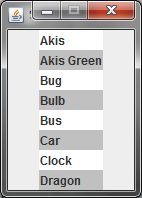
\includegraphics{3.Prototype/Add_Vindue}
    \caption{Add Vindue 3.Prototype}
    \label{add3}
\end{figure}
\begin{figure}[ht]
\centering
	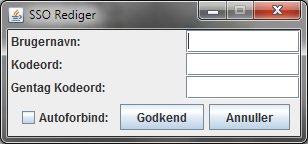
\includegraphics{3.Prototype/Edit_Vindue}
    \caption{Edit Vindue 3.Prototype}
    \label{edit3}
\end{figure}
\begin{figure}[ht]
\centering
	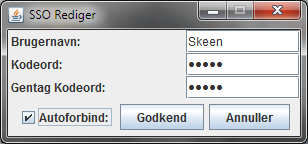
\includegraphics{3.Prototype/Edit_Vindue_Info}
    \caption{Edit Vindue Info 3.Prototype}
    \label{edit3info}
\end{figure}
\begin{figure}[ht]
\centering
	\includegraphics{3.Prototype/TrayIcon}
    \caption{Tray Icon 3.Prototype (2. ikon fra venstre)}
    \label{tray3}
\end{figure}
\begin{figure}[ht]
\centering
	\includegraphics{3.Prototype/TrayIconMenu}
    \caption{Tray Icon menu 3.Prototype}
    \label{tray3menu}
\end{figure}

\begin{figure}[ht]
\centering
	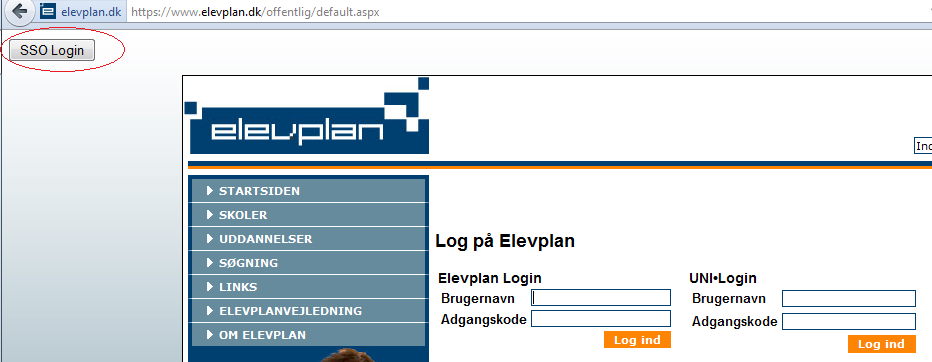
\includegraphics[height= 150px]{3.Prototype/SSO_Login_Button}
    \caption{SSO Login Button 3.Prototype}
    \label{ssologinbutton}
\end{figure}
\begin{figure}[ht]
\centering
	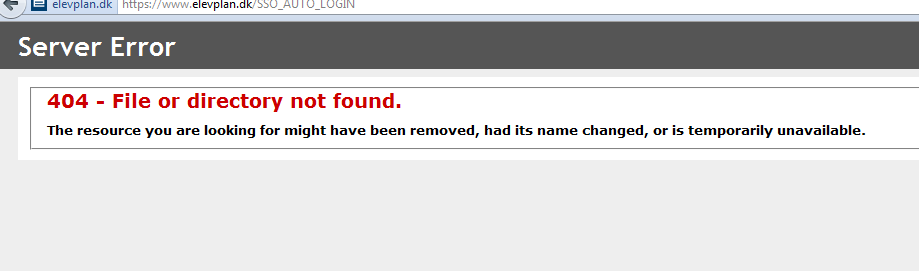
\includegraphics[height= 100px]{3.Prototype/404}
    \caption{Fejl: 404 3.Prototype}
    \label{fejl404}
\end{figure}

\begin{figure}[ht]
\centering
	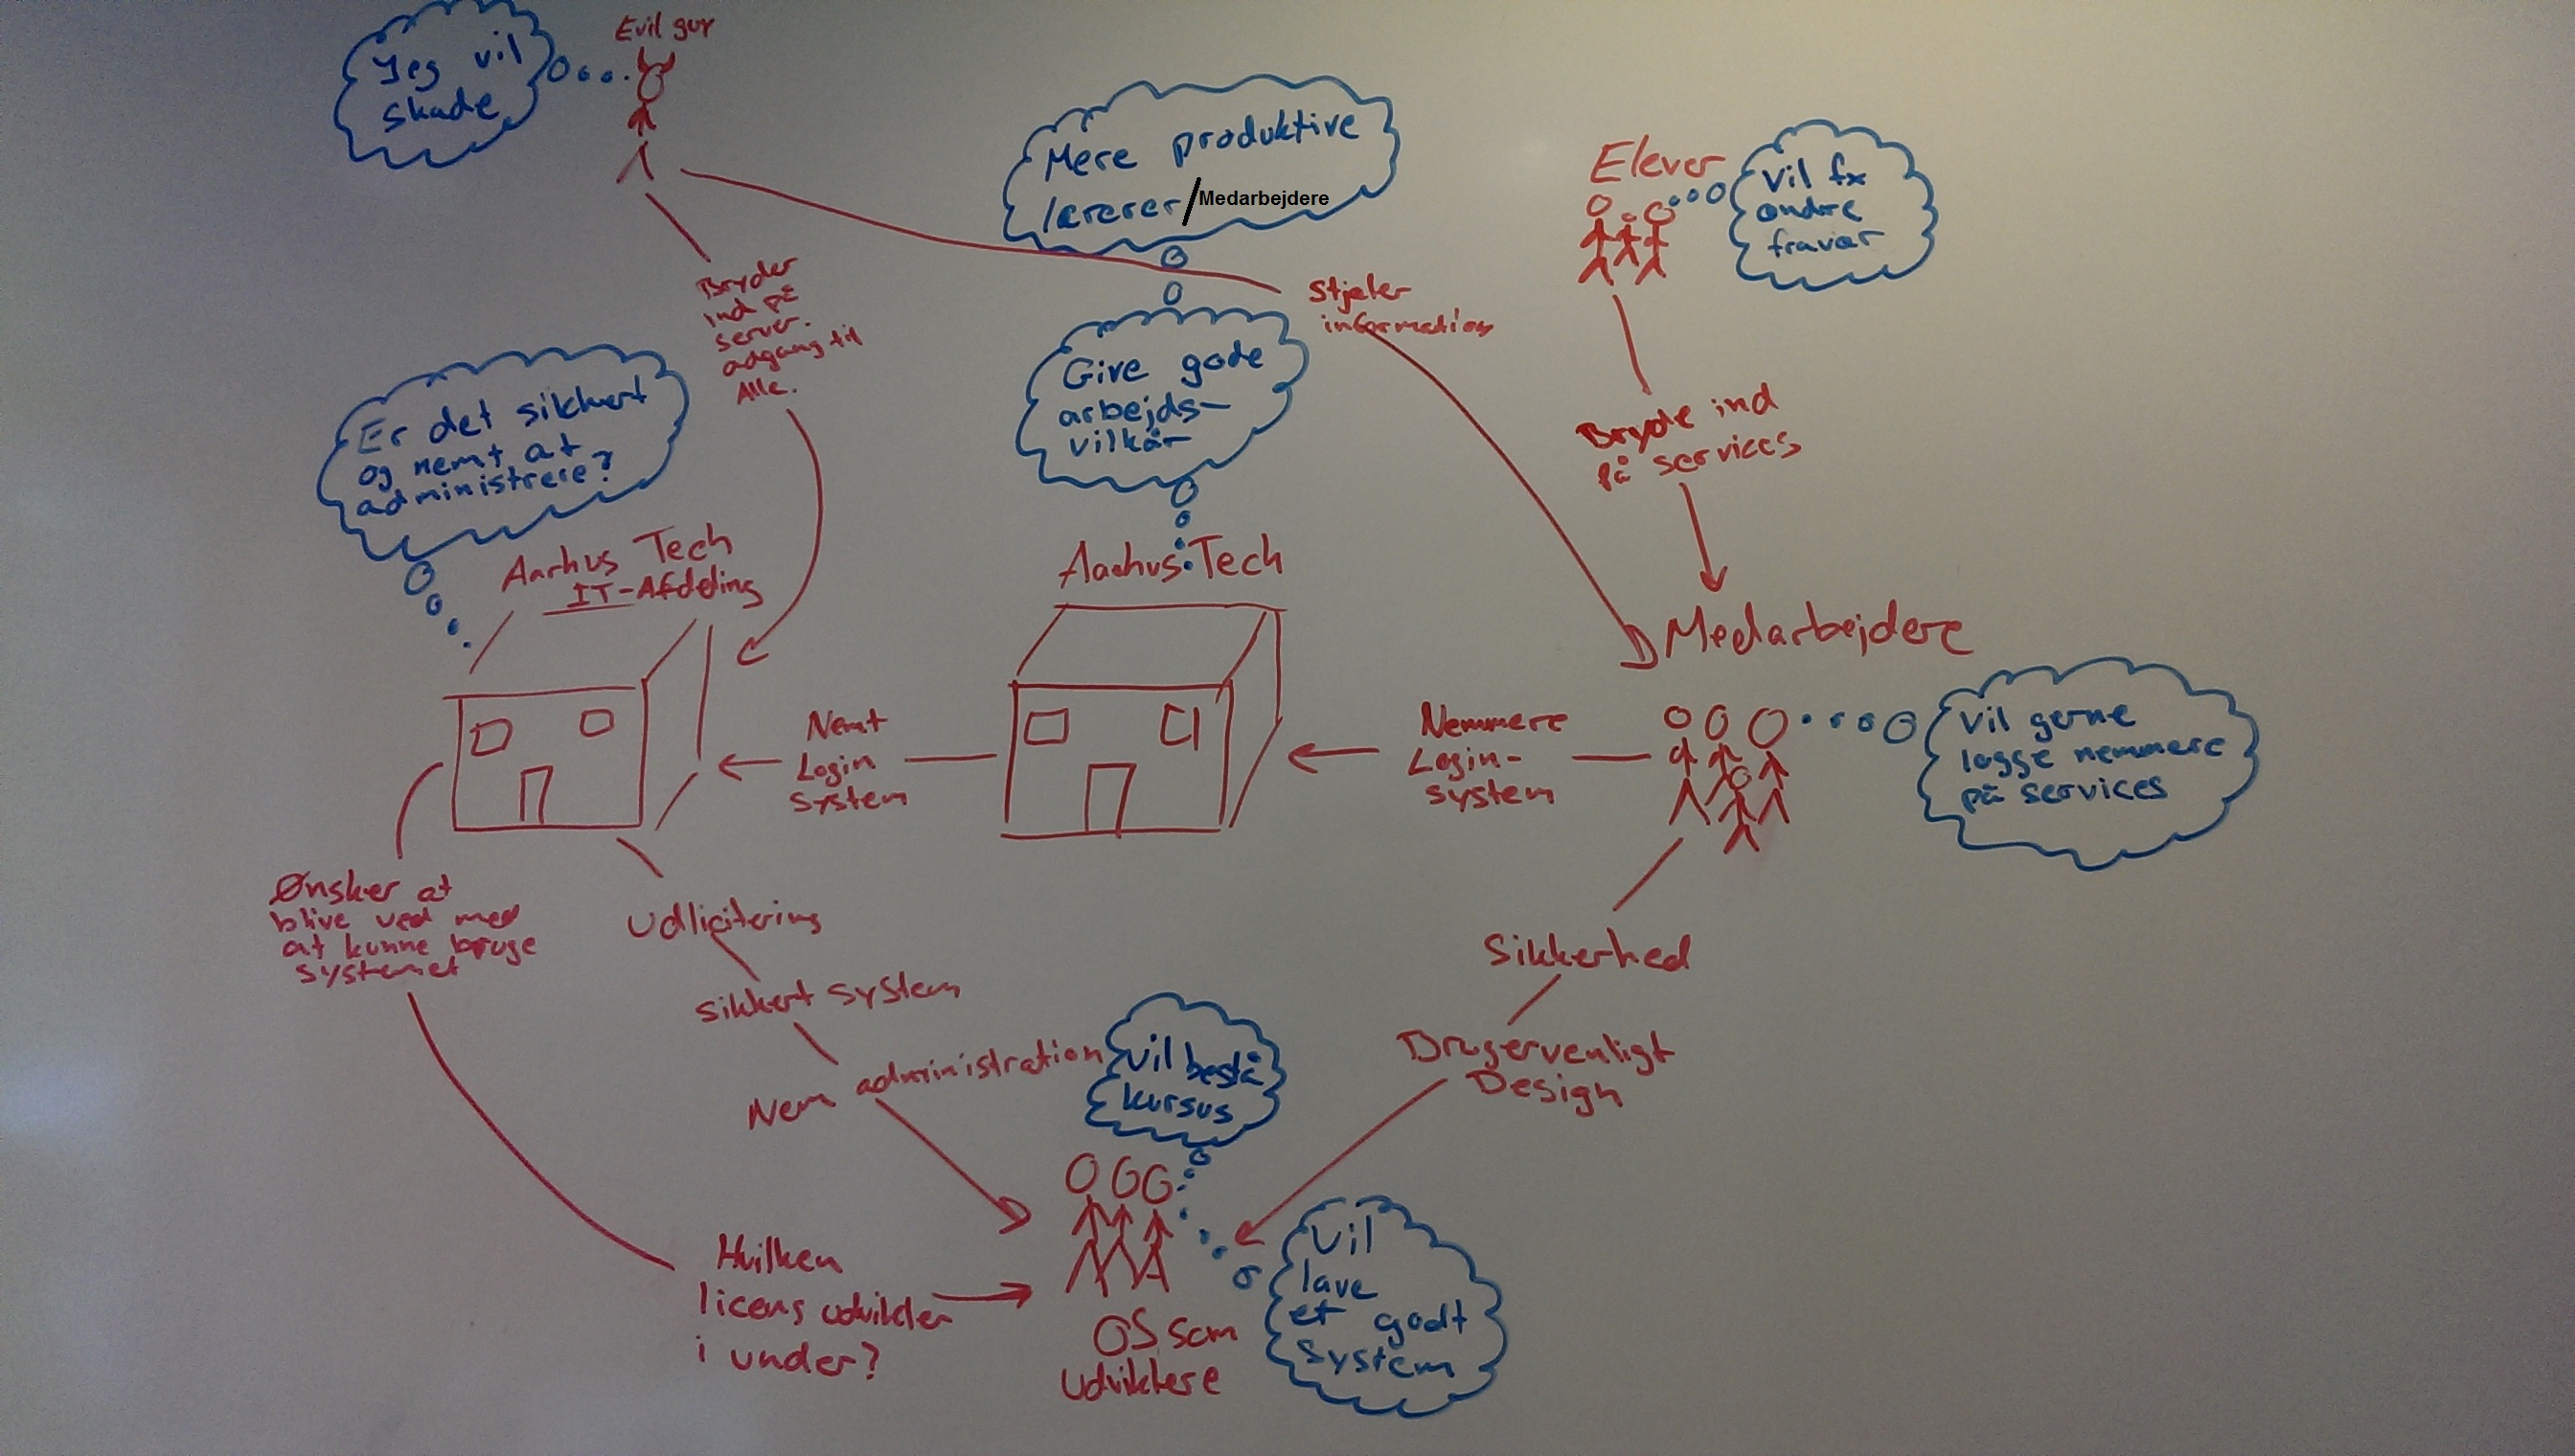
\includegraphics[height= 235px]{Rich_Picture}
    \caption{Rich Picture}
    \label{richpicture}
\end{figure}

\FloatBarrier
%interview pdfs
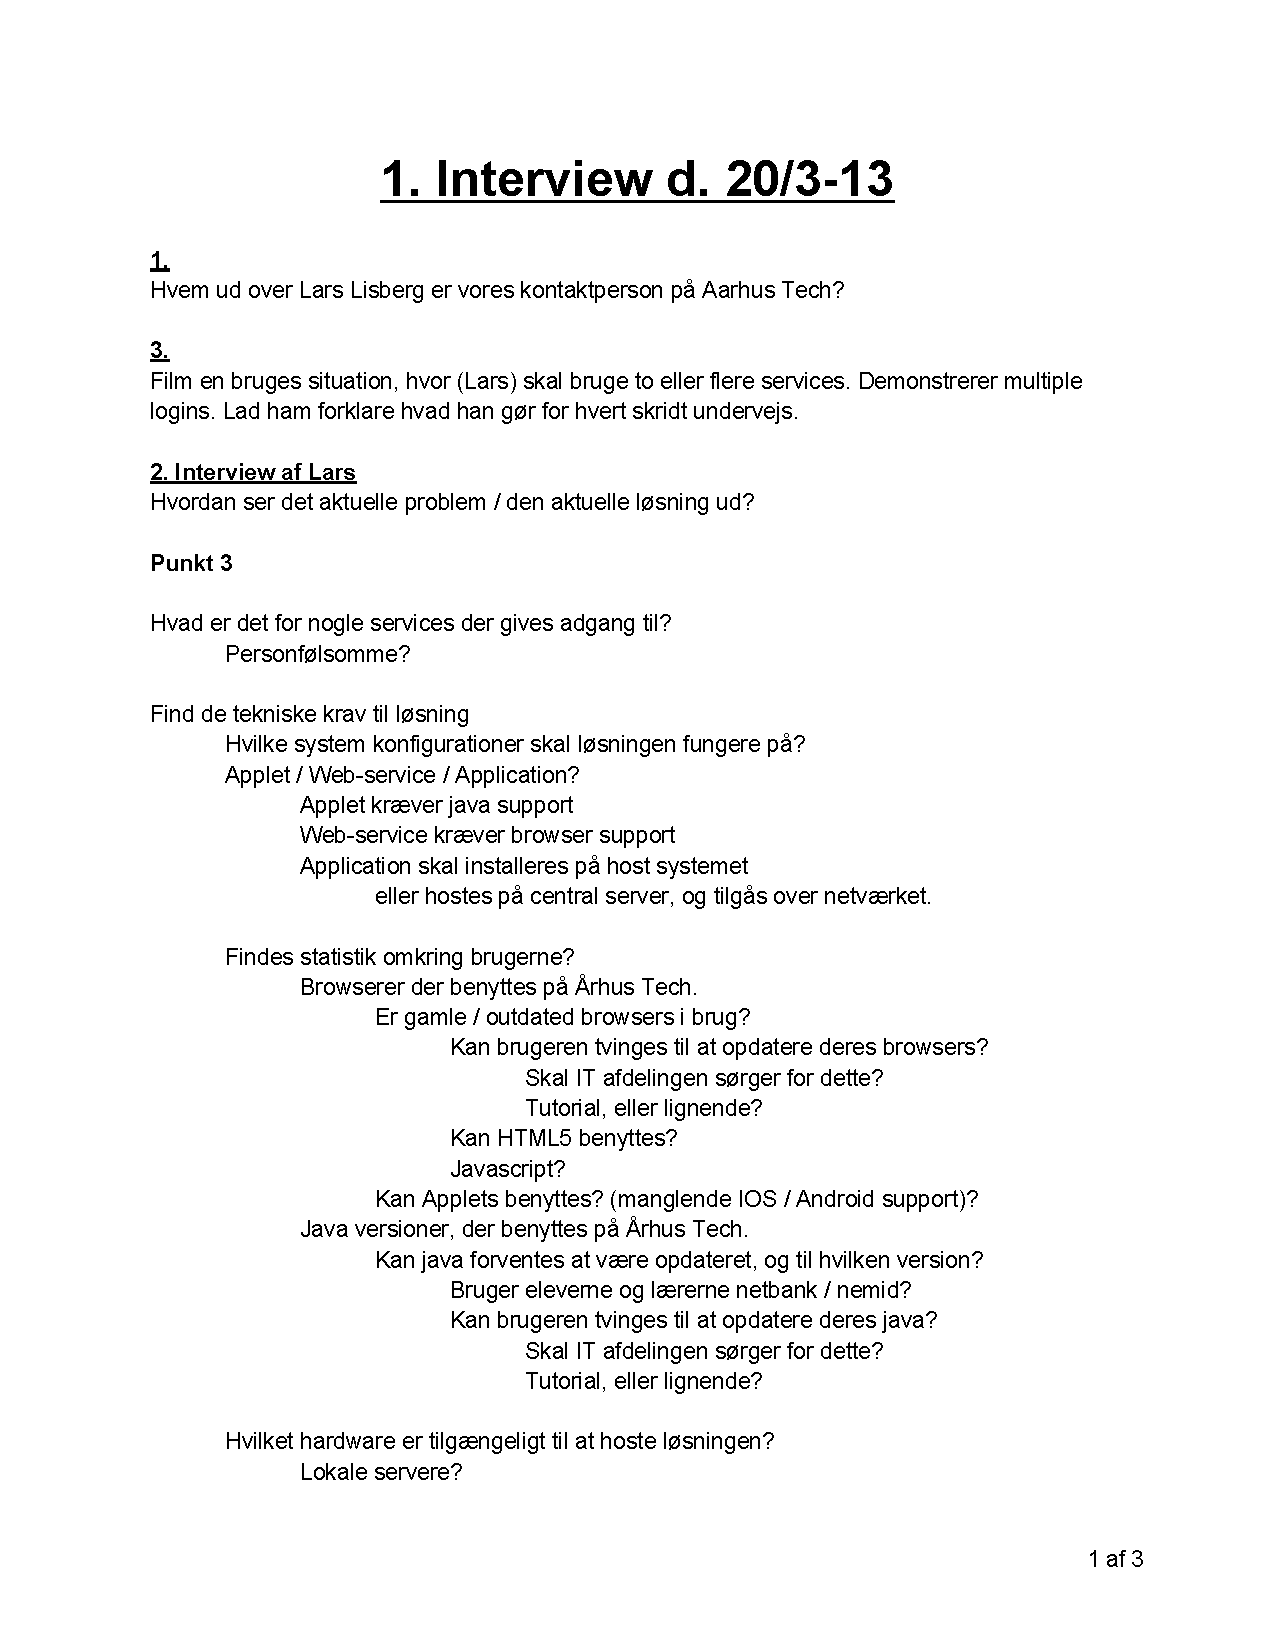
\includepdf[pages={1,2,3}]{gfx/1_interview.pdf}
\label{interview1}

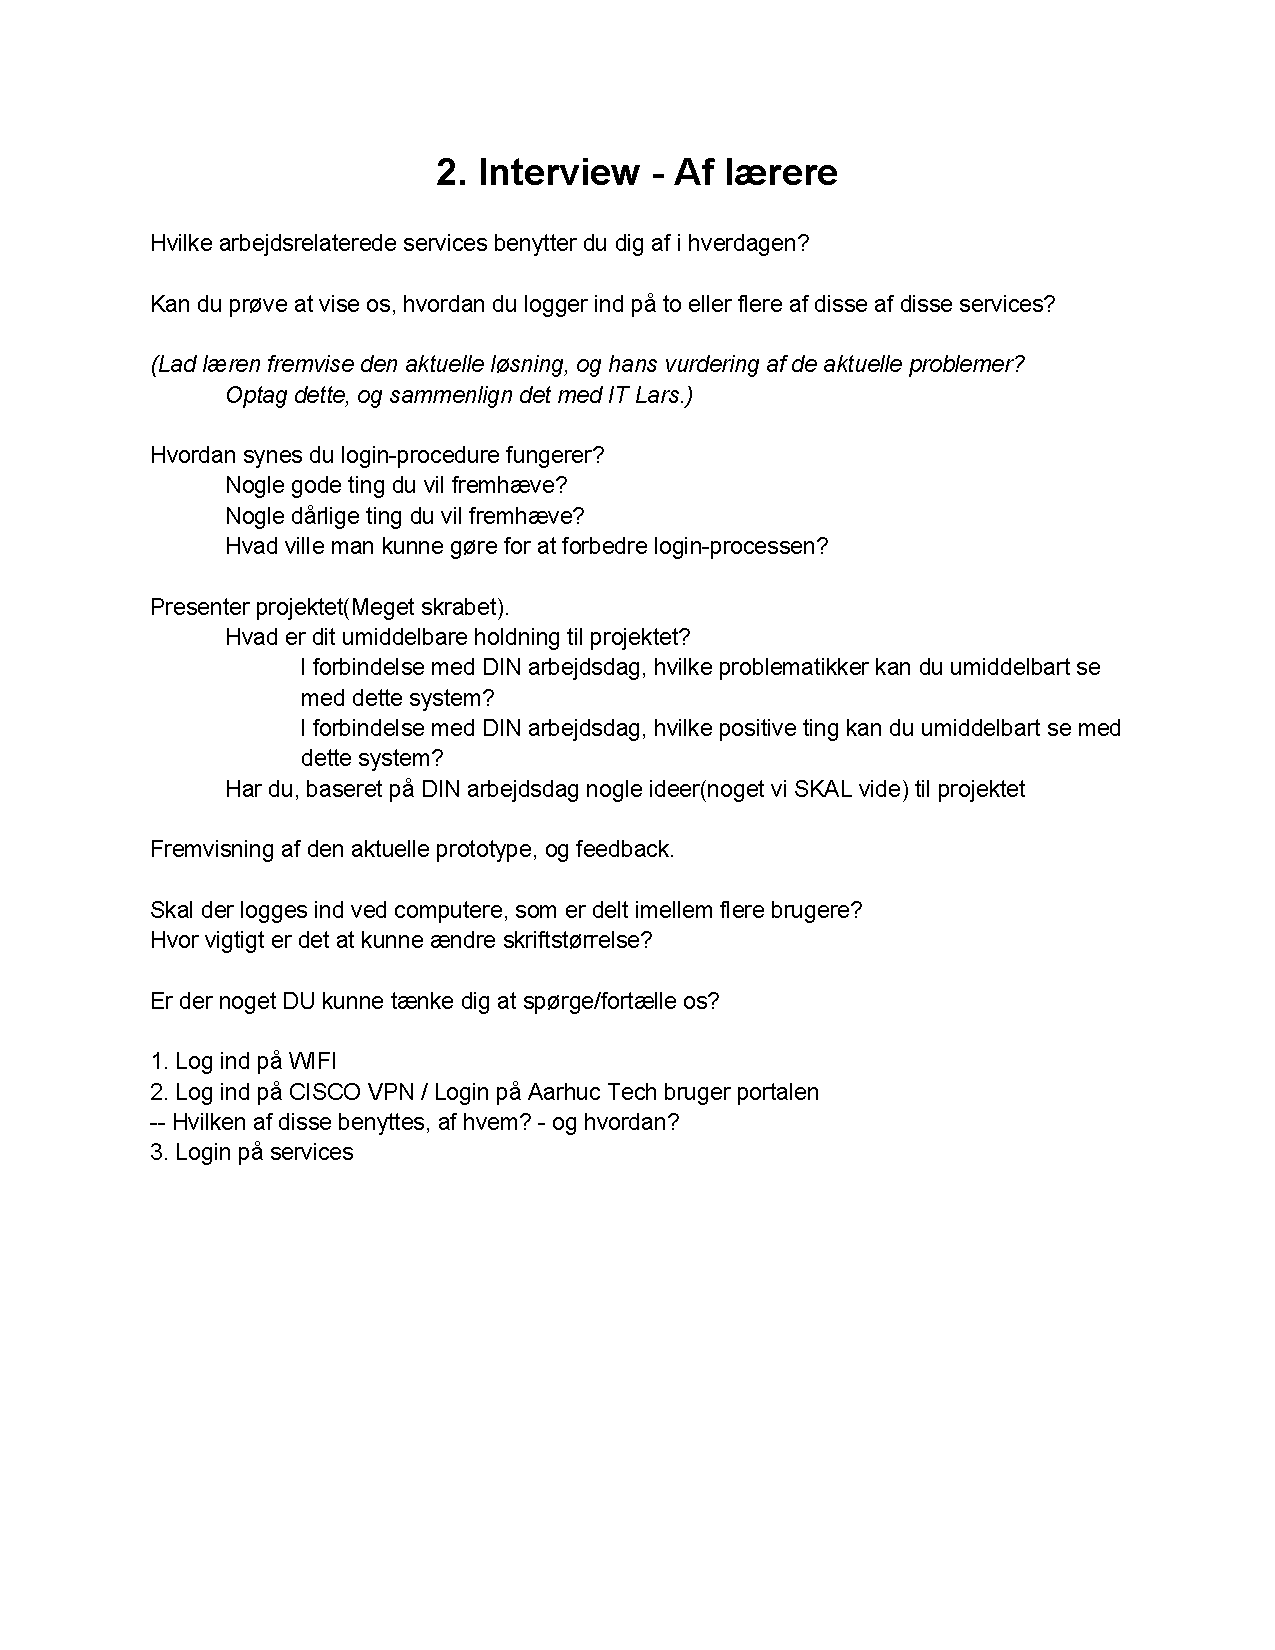
\includepdf[pages={1}]{gfx/2_interview.pdf}
\label{interview2}

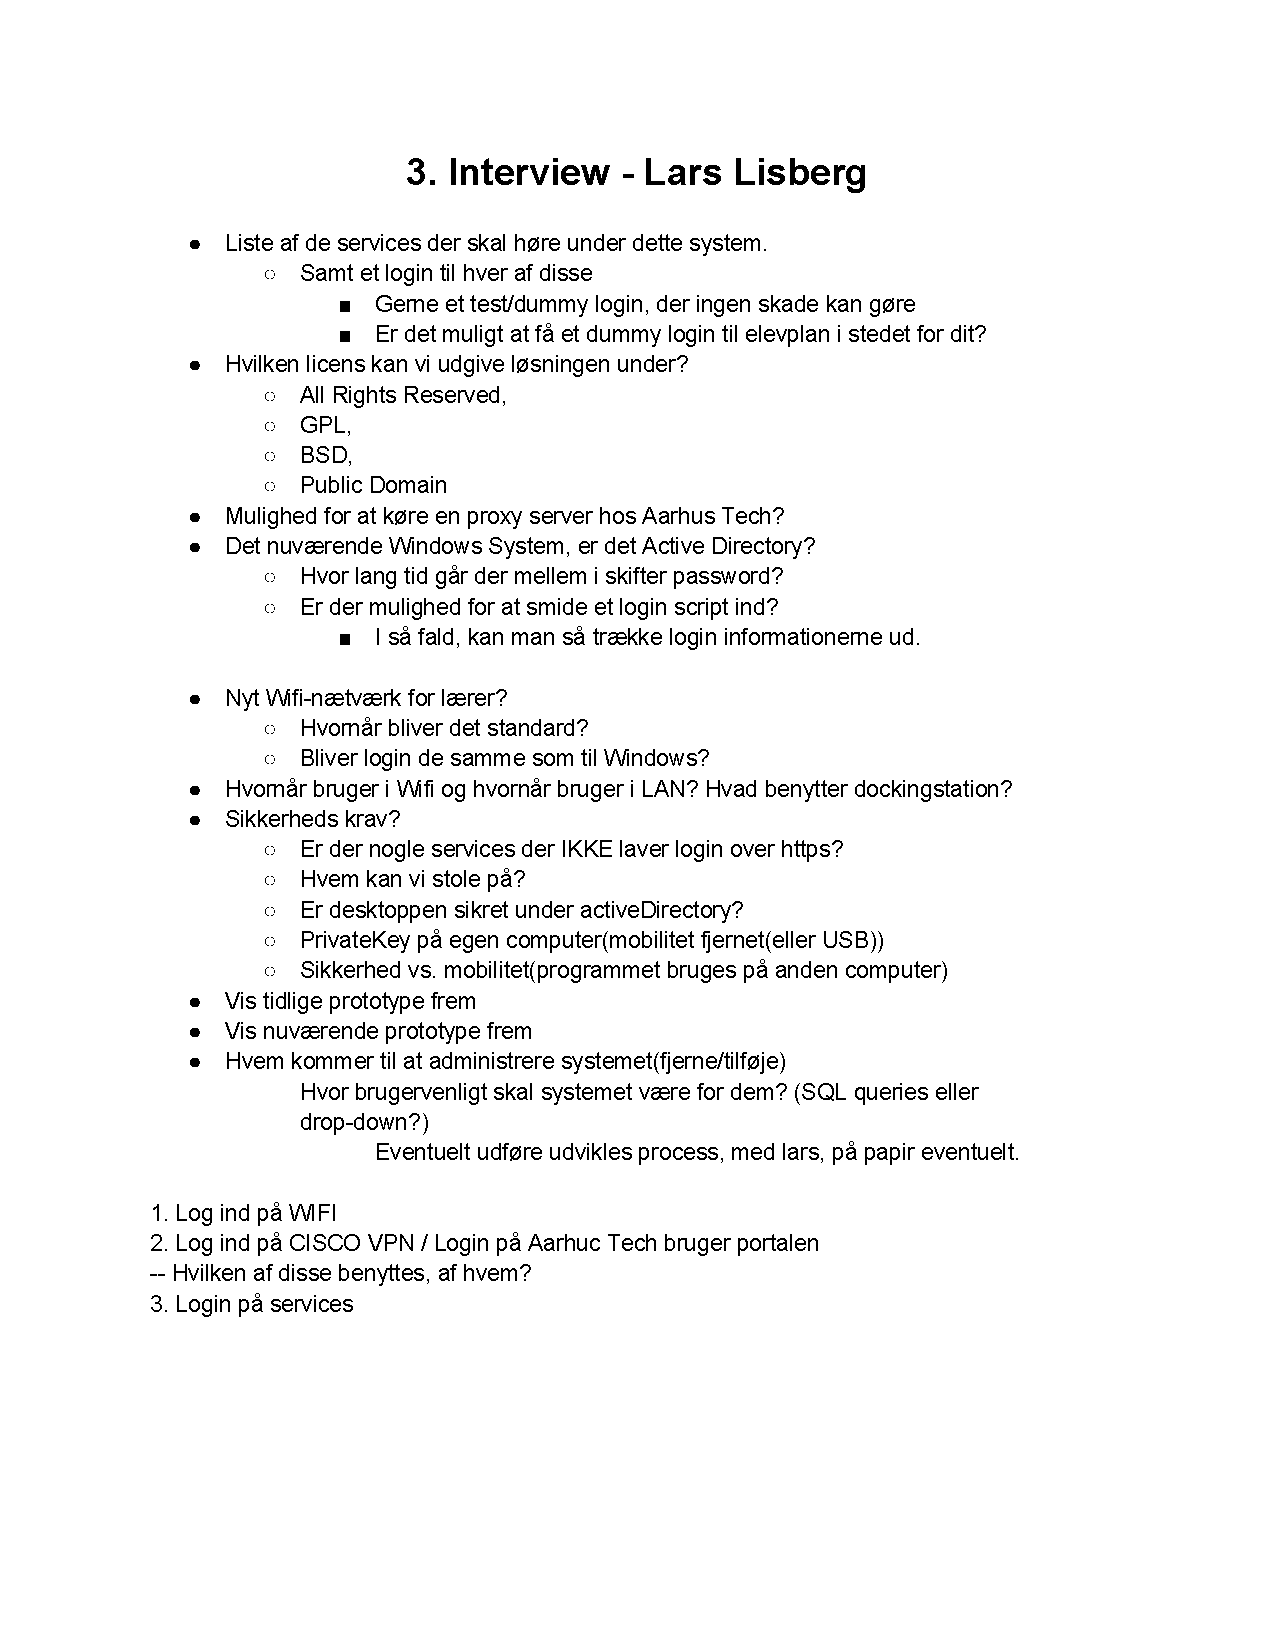
\includepdf[pages={1}]{gfx/3_interview.pdf}
\label{interview3}

 

% Setup bibtex
% \newpage
% \bibliography{FVTITDAT2012,OTHERS}

% that's all folks
\end{document}

